%%-----------------Chapter 6---------------------------
% \documentclass[../UNBThesis2.tex]{subfiles}
\setlength{\parindent}{2em}
%%%%%%%%%% NUMber of centrers + run time -memory.....
%%%%%%%% winodow length+ all validation metrics




% %\colorbox{yellow}{one week --AP/ Kmeans(same week)--> first week int }
% % \colorbox{yellow}{one day position/count(same day)} %Friday, October 30, 3987 --monday(first day of inter)i
% % \colorbox{yellow}{update hourly one day(same day -5/1)} --> one day AP 
% \colorbox{yellow}{summary plot -->waterfall evolution - one week po cou tim } cluster center???
% \colorbox{yellow}{LBAP -one week }
% % \colorbox{yellow}{DSAP one week}
% \colorbox{yellow}{streaming Kmeans --one week???}

% \colorbox{yellow}{DSAP 3 seprate month}
% \colorbox{yellow}{Streaming Kmeans 3 sep month}
% % \colorbox{yellow}{one month Kmeans}
% \colorbox{yellow}{waterfal one month --> x: month y: position z: number of people }

% \begin{document}
\chapter{Discussion of the Results}

In this Chapter, the main clustering results from applying stream clustering using the data streams generated from both experiments are presented to discuss the strengths and weaknesses of the proposed DSAP algorithm. 
%of AP and discuss how DSAP provides potential solutions to these.
%\subsubsection{Comparison between DSAP and streaming K-means Phase}: The aim is to demonstrate the relevance of the proposed DSAP approach compared to streaming K-means algorithm. very important to explain why streaming kemans: - difficult to find available source code from previusouly proposed stream AP, etc...online)no offline) - no window
% \section{Validation of DSAP Algorithm}
% \section{Experimentation on Dataset}
% \section{experimental results}
% \section{Experiments with real-world e-counter data}

% time interval used is one hour for ecounters
% time interval used was 10 minutes for wifi



% to show the results:

% Ecounters 

% descriptive: entire experiment/distribution: Fig 6.1. daily total number of counts for the entire experiment time. White: two weeks off for the March break, 6.2 gree in friday, orange is tuesday, fig 6.3, fig 6.4,  fig 6.5 (we need the other two blocks), maybe 6.6 is not needed(Nasrin, if you find an interpretation that is relevant)>>>>> we have all these figures, but the conclusion is that the campaign has not worked, not motivated people to take the stairs... time of the experiment was the end of the semester...

% AP (weekly patterns)

% fig. 8: Comparison of cluster patterns found during one week of before, during, and after intervention
% clusters for one week of data ( data points, and numbers show how many data points a cluster has, colour represents the clusters) before the intervention 
% one week of data before intervention
% you will add
% one week of data during the intervention
% one week of data after the intervention

% Kmeans >>>  OUT
% fig 6.9: same week as before, same data as fig 8, but running kmeans


% DSAP
% CLUSTER EVOLUTION
% fig.7: show the hourly evolution of the micro-cluster for each time window for one day during intervention.
% fig 20: will show the monthly evolution through the beginning, during, and after the experiment. 

% EVALUATION (PERFORMANCE, QUALITY)
% New Figure
% one week of data before the intervention
% one week of data during the intervention
% one week of data after the intervention
% same weeks that you have used in AP Fig 8
% to show how many micro-clusters belong to a macro-cluster
% if it is too complicated, make a table.
% PURPOSE: With AP and DSAP: we found the same patterns or not???

% Combine the three tables:highlight the table with the results that we are going to discuss in detail
% Table 6.1 : one week before the intervention
% Table 6.2  : one week during
% Table 6.3 : one week after
% the same weeks that have been used for the figures
% PURPOSE: to know if get similar performance and quality results for the 3 weeks. = to prove that DSAP is robust




%--------------------------
%%%%%%%%%%%%%%%%%%%%%%%%%%%%%%%%%%%%%%%%%%%%%%%%%%%%%%%%%%%%%%%%%%%%%%%%%%%%%%%%%%%%%%%%%%%%%%%%%


%In this chapter, data from the e-counter and WiFi Indoor Localization experiments are analyzed using traditional and streaming clustering algorithms to gain insights into the measurements. We demonstrate the strengths and weaknesses of AP and discuss how DSAP provides potential solutions to these.
% Data stream clustering results are also compared with the results from the streaming K-means algorithm. 

% Both the experiments provide information regarding occupant's behaviour and movement within a confined space. The details of the experiments and the analysis tools have already been discussed in the last two Chapters. In the following sections, the data sets will be explained in detail, and the patterns identified by the clustering methods will be analyzed.

 
\section{Behavioural Intervention Experiment} 

The streaming cluster analysis was aimed at finding any evolutionary patterns in stair usage due to an educational intervention campaign. The clustering results were generated using three months of the experiment, which were named as before, during, and after the intervention.


\subsection{Spatio-temporal Data Patterns}

%The people counter sensors located at the stairs of the Tonsley building log several parameters.

The most relevant measurements for this cluster analysis were the location of people counter sensors at the Tonsley building and the number of people passing through these sensors. The landmark time window of one hour was used to accumulate the data streams. Figure \ref{updown} illustrates the daily stair usage patterns. The three months named as before intervention, during the intervention, and after intervention are highlighted in purple, blue, and yellow shaded regions, respectively. It is quite apparent that more people preferred taking the stairs to go down rather than up. An expected low usage of stairs is also observed on the weekends. The mid-semester break from April 15-28 was excluded from the analysis as the measurements made during this period represented anomalous behavior. 

\begin{figure}[b]
    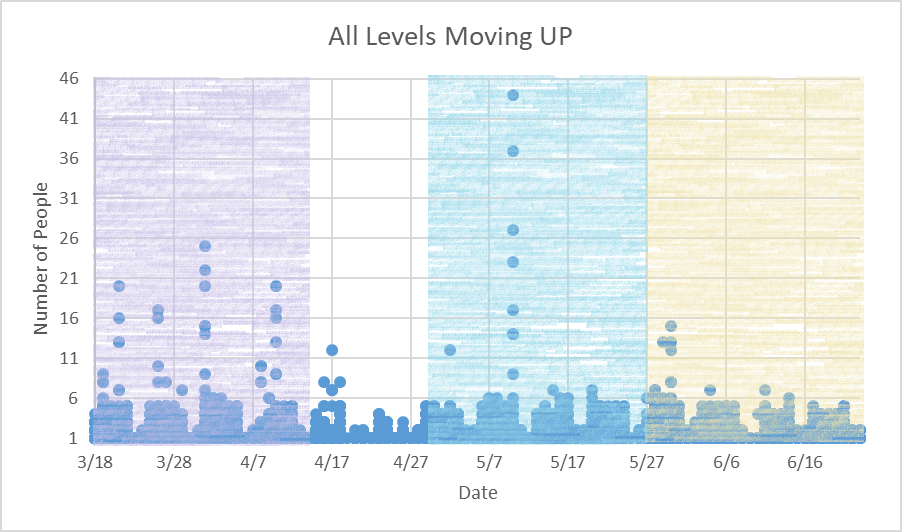
\includegraphics[width=0.5\textwidth]{image/Chapters/Chapter6/up.png}%\hfill
    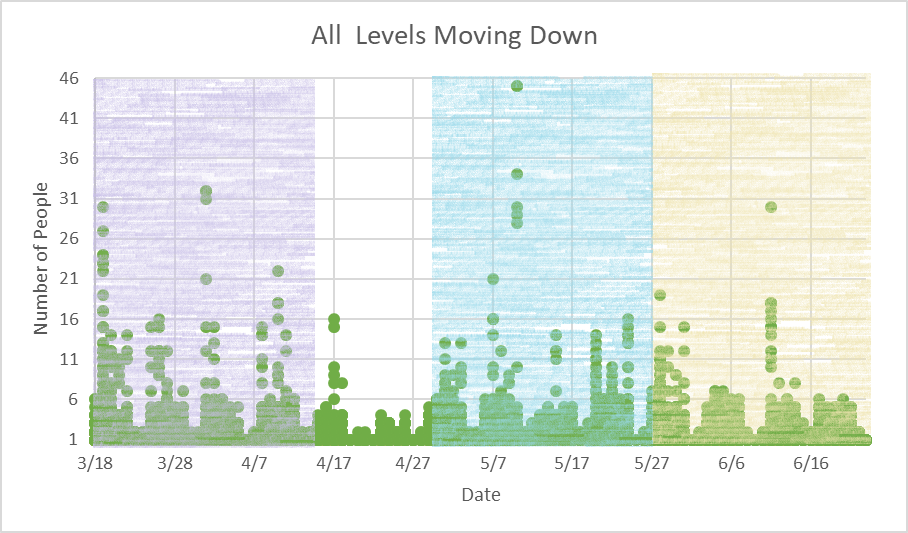
\includegraphics[width=0.5\textwidth]{image/Chapters/Chapter6/down.png}
    % \\[\smallskipamount]
    \caption{Total number of people using the stairs: before intervention month (purple), during intervention month (blue), and after intervention month (yellow)}
    \label{updown}
\end{figure}

%These accurate integer-valued parameters not only indicate the number of people occupying any particular floor but also accurately determine the number of people using the stairs in any particular direction.

%The entire dataset split by the direction of stair use represents 

To gain further insights into the data, Figure \ref{3mon} shows the number of people using the stairs (both up and down) for each month of the experiment. No discernible differences could be found in these patterns that were observed between the weekdays for one month of data collected before, after, and during the intervention. The weekends as expected, reported count values orders of magnitude smaller than the weekdays. Although the overall trend of the number of people using the stairs at each level remains consistent for the three months, one peak of stair usage occurred on Monday April 1, before the intervention, another peak occurred on Friday May 10, during the intervention and happened again on Tuesday June 11 after the intervention campaign has ended.
After a closer inspection of the data, it was found that on May 10, a group of students went up around 12:06 pm, and presumably, the same group came down at 12:23 pm. This led to an increase in the measured count across many levels, whether this alone accounts for the increase in the accumulated count values for the entire month after the intervention. No particular event was found to justify other peaks. 


\begin{figure}[!htbp]
\centering
    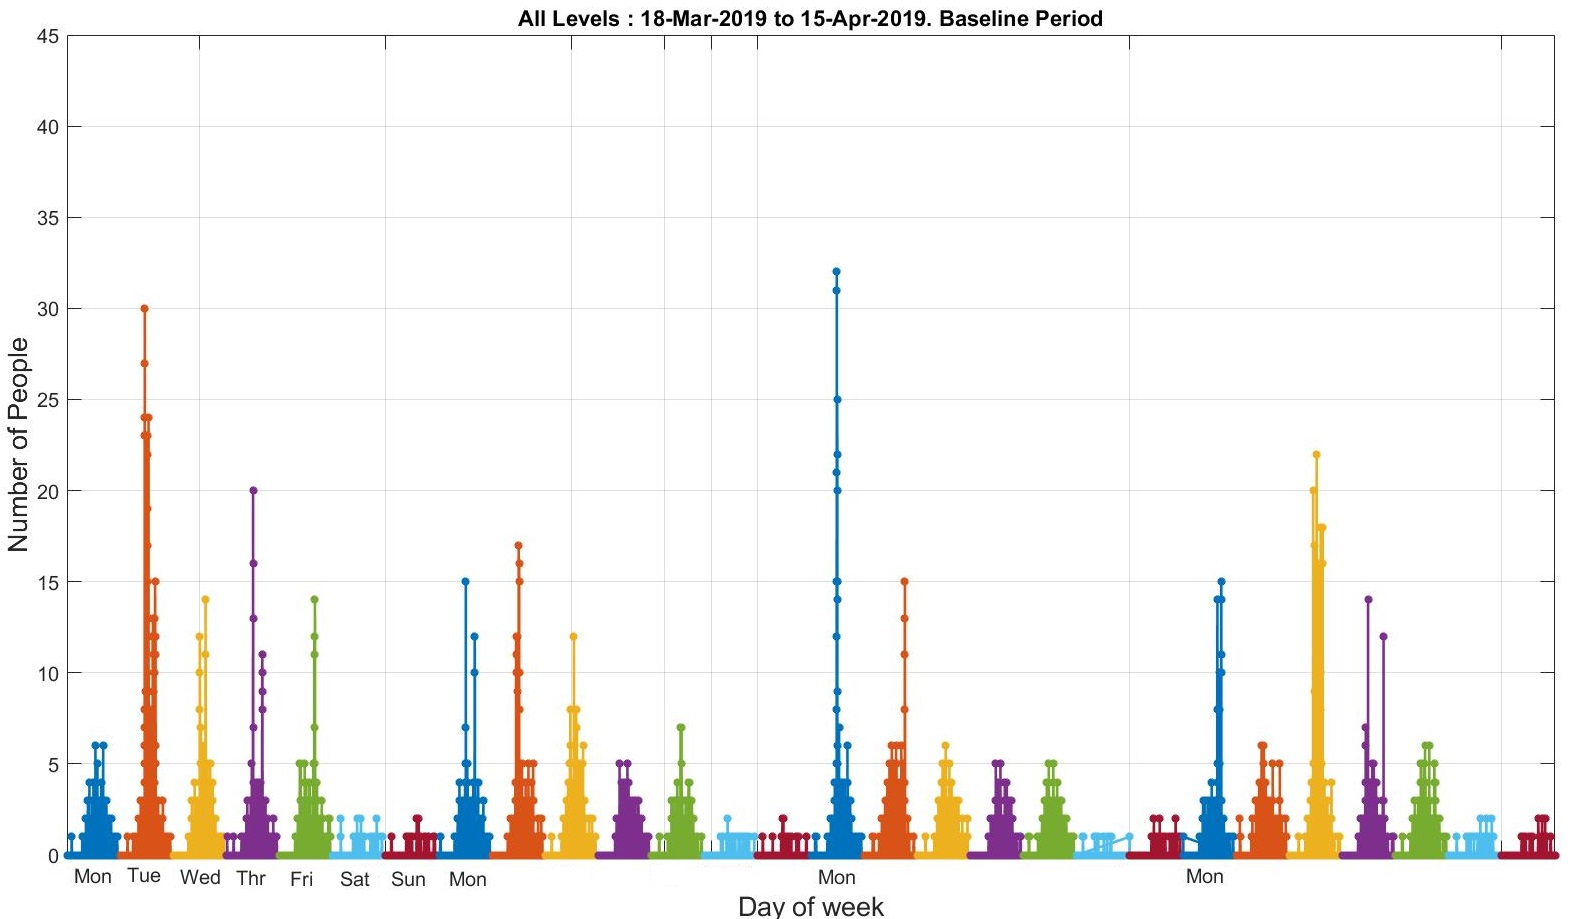
\includegraphics[width=0.65\textwidth]{image/Chapters/Chapter6/18-Mar-2019Base.jpg}
    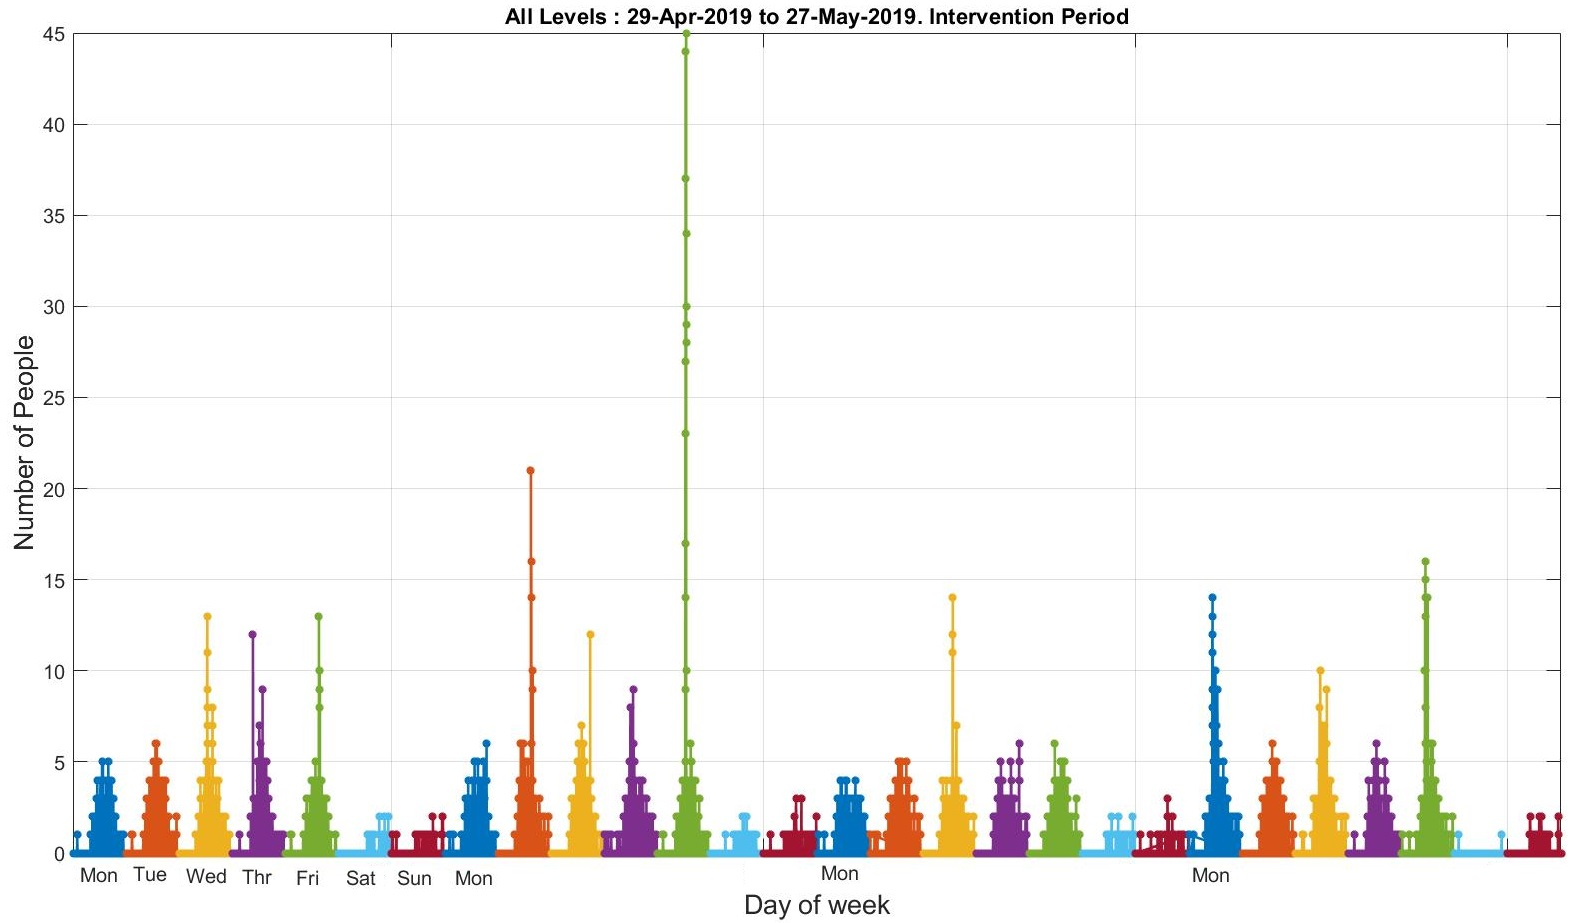
\includegraphics[width=0.65\textwidth]{image/Chapters/Chapter6/29-Apr-2019Int.jpg}
    % \hfill
    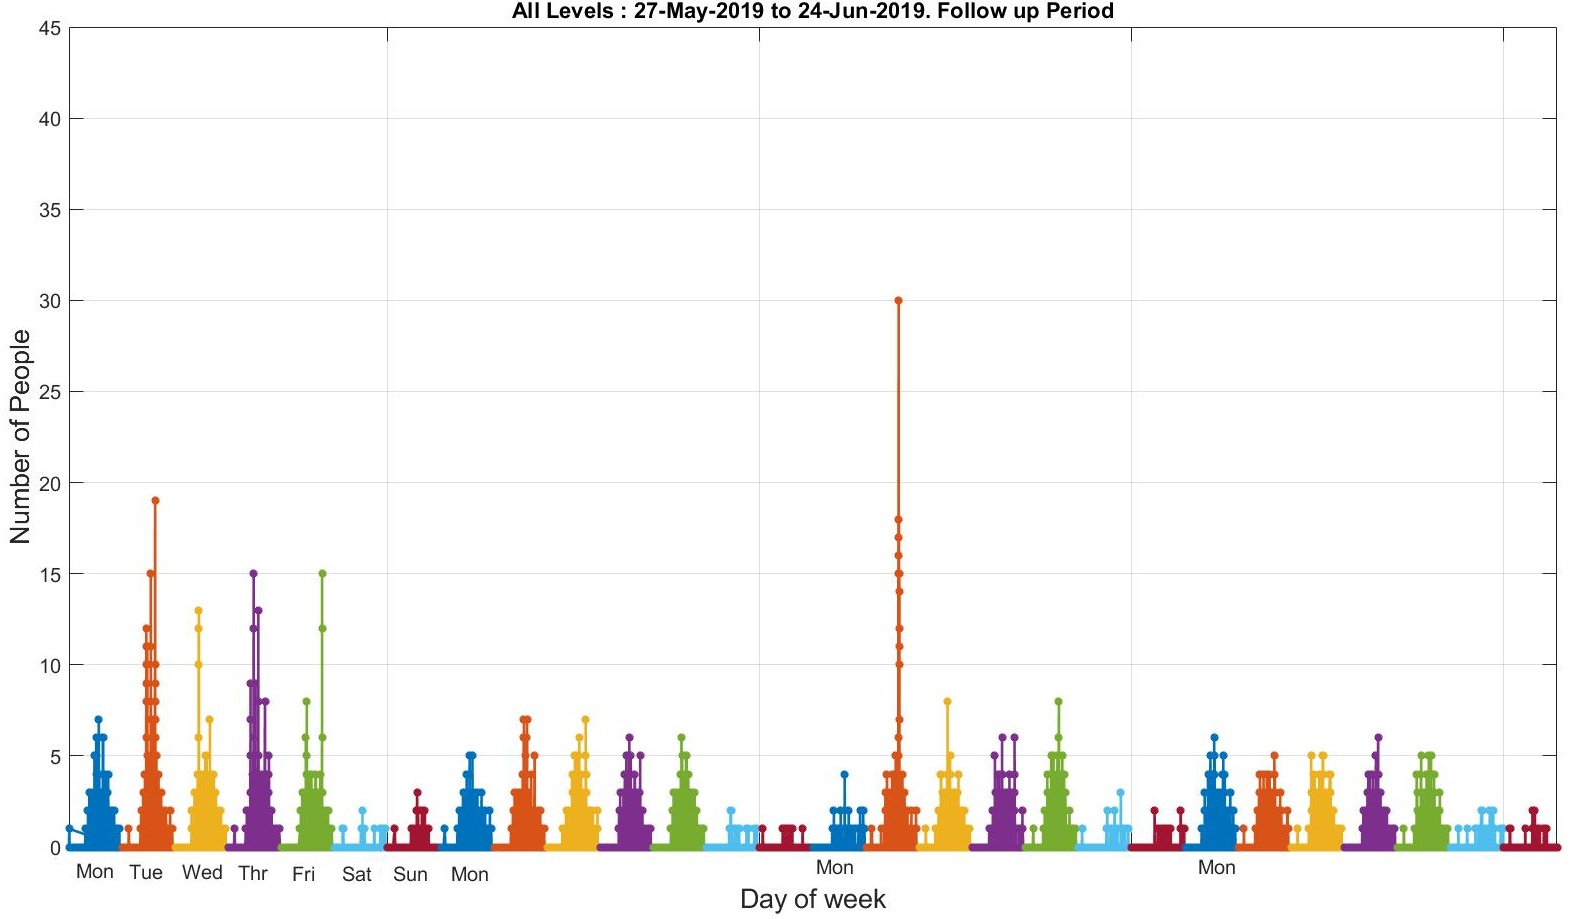
\includegraphics[width=0.65\textwidth]{image/Chapters/Chapter6/27-May-2019Follow.jpg}
    % \\[\smallskipamount]
    \caption{Weekly patterns of stair usage before, after and during intervention: Sunday (light blue), Monday (red), Tuesday (dark blue), Wednesday (orange), Thursday (yellow), Friday (purple), Saturday (green)}
    \label{3mon}
\end{figure}


%\todo[inline]{Nasrin: write down the exact dates when the peaks have occured } 

A dynamic pattern behaviour was also observed on an hourly basis for each month of the experiment, as shown in Figure \ref{spa2}. The usage peak is around noon for most of the weekdays, most probably due to the lunch break. The people count is asymmetric on both sides of the peak, with more people using the stairs on Tuesday afternoons during all months of the experiment. Overall the month before the intervention campaign seems to have recorded the highest usage than the following months. By looking at this trend, our preliminary hypothesis is that the intervention campaign has not generated the expected impact on motivating people to take the stairs. Therefore, the clustering results play a significant role in testing this hypothesis.  % these observations can also be made from the next figure.

\begin{figure}[tbp]
    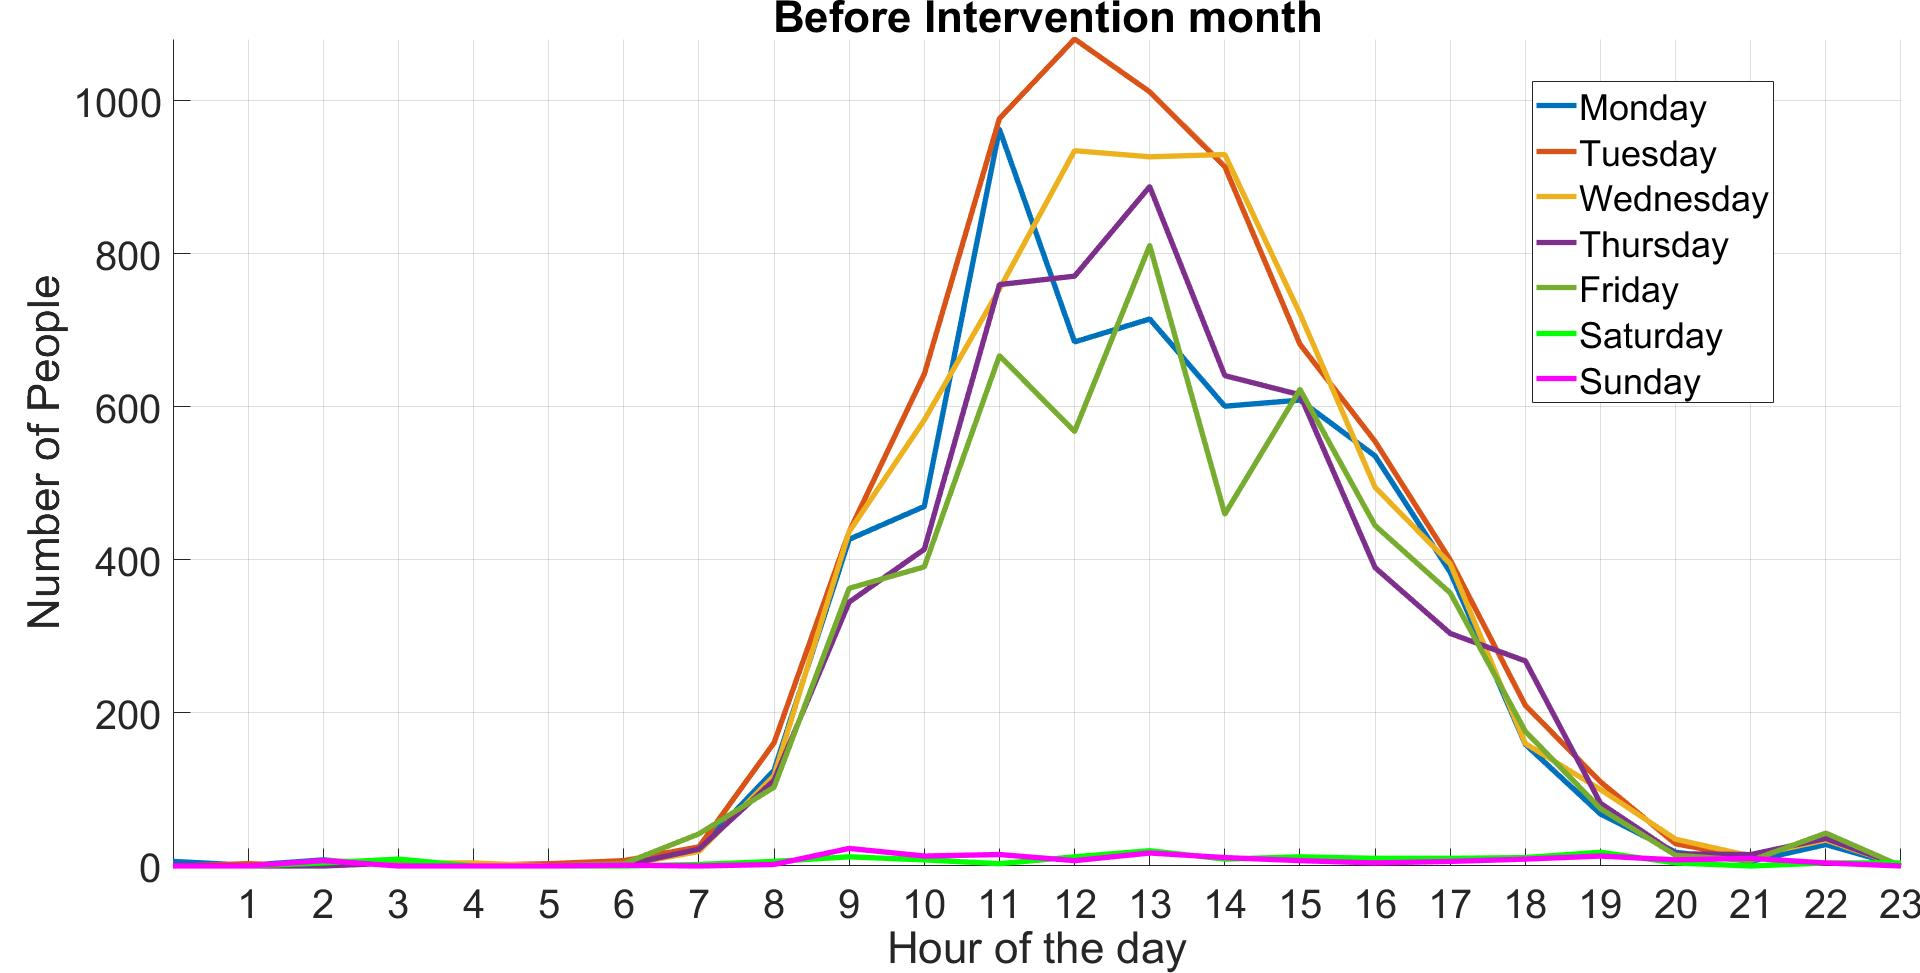
\includegraphics[width=.49\textwidth]{image/Chapters/Chapter6/aggWeekPre.jpg}%\hfill
    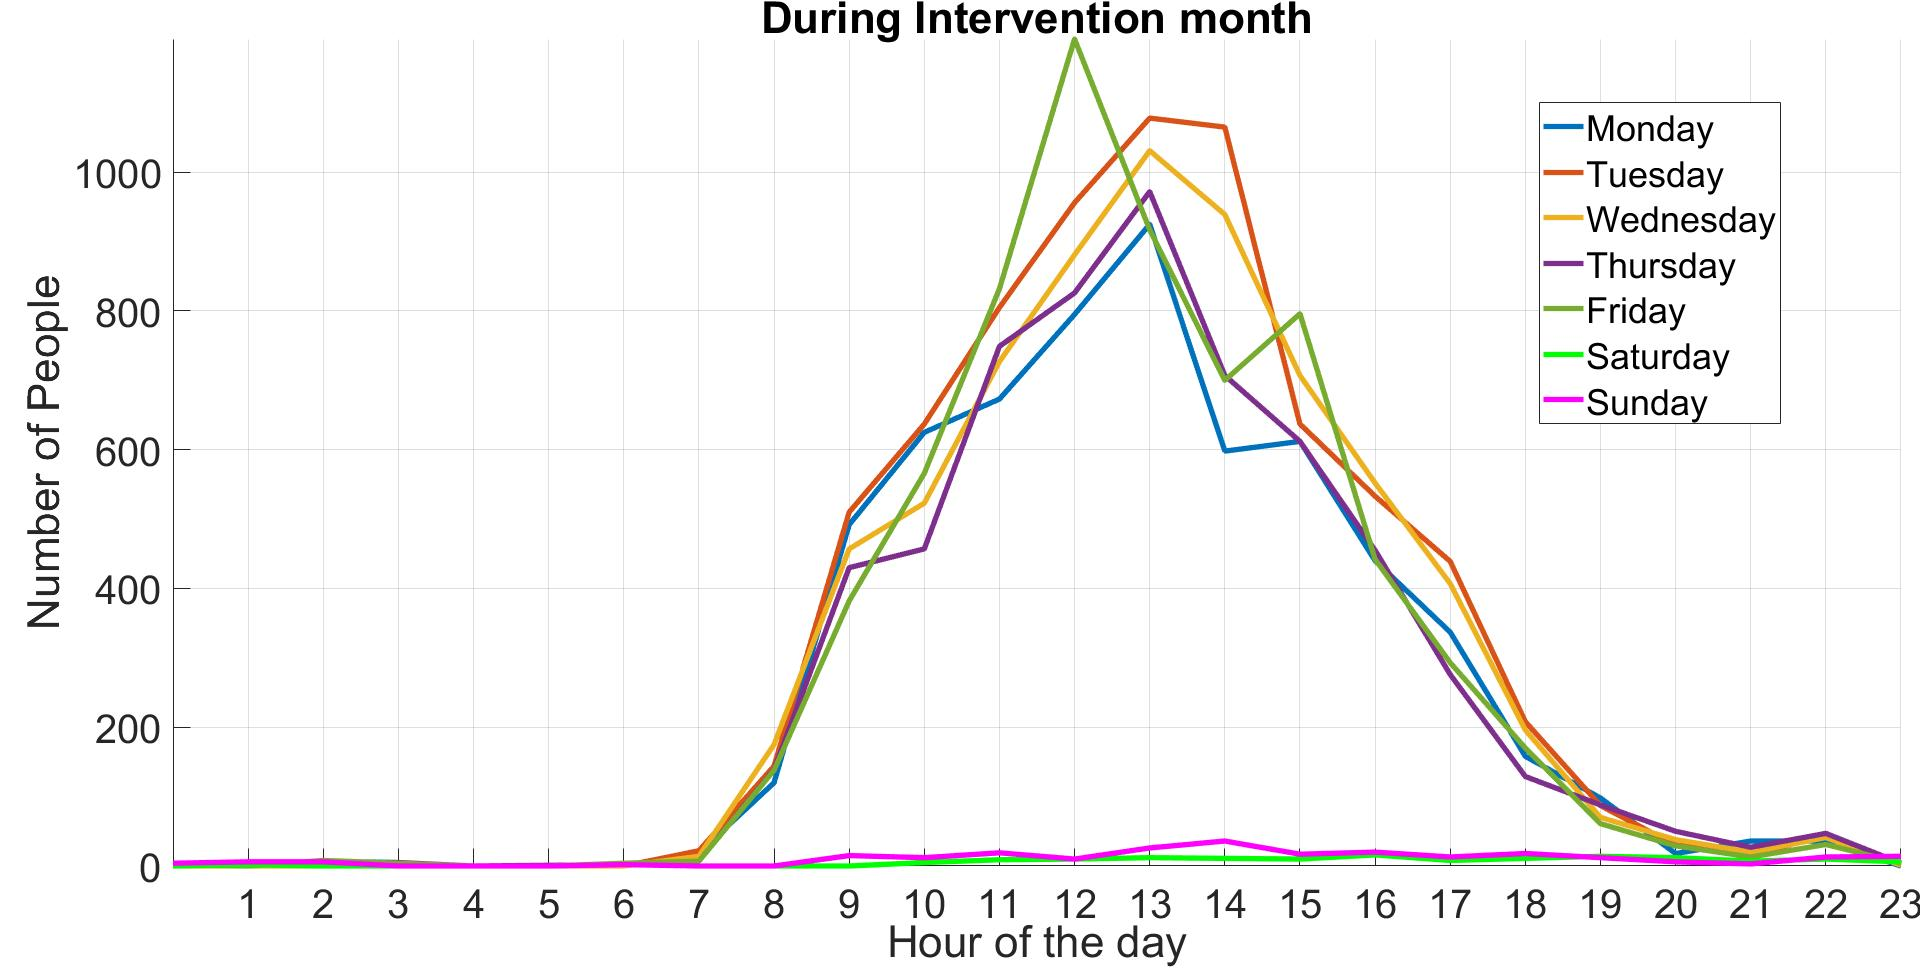
\includegraphics[width=.49\textwidth]{image/Chapters/Chapter6/aggWeekInt.jpg}\hfill\centering
    \includegraphics[width=.49\textwidth]{image/Chapters/Chapter6/aggWeekpost.jpg}
    %\\[\smallskipamount]
    \caption{Hourly stair usage patterns for each month: before (top), during (middle), and after (bottom) intervention}
    \label{spa2}
\end{figure}



%The aggregated weekly distribution of stair usage for the three periods is plotted in Figure \ref{spa2}. 

% No discernible differences could be found in the distribution patterns that were observed between the weekdays for one month of data collected before, after, and during intervention (Figure \ref{spa2}). The weekends as expected reported count values orders of magnitude smaller than the weekdays. Although the overall trend of the number of people at each level remains consistent for the three months, one peak of stair usage was occurred on Tuesday DATE HERE before in the intervention, another peak occurred on Monday DATE HERE during the intervention, and happened again on Wednesday DATE HERE after the intervention campaign has ended. No particular event was found to justify these peaks. 

% \todo[inline]{Nasrin: write down the exact dates when the peaks have occured }
%but an increase at each level is observed during the month of intervention which warrants further study.NOT SURE WHAT IS MEANT HERE


\begin{figure}[htb]
\centering
    \begin{minipage}[b]{0.5\textwidth}
    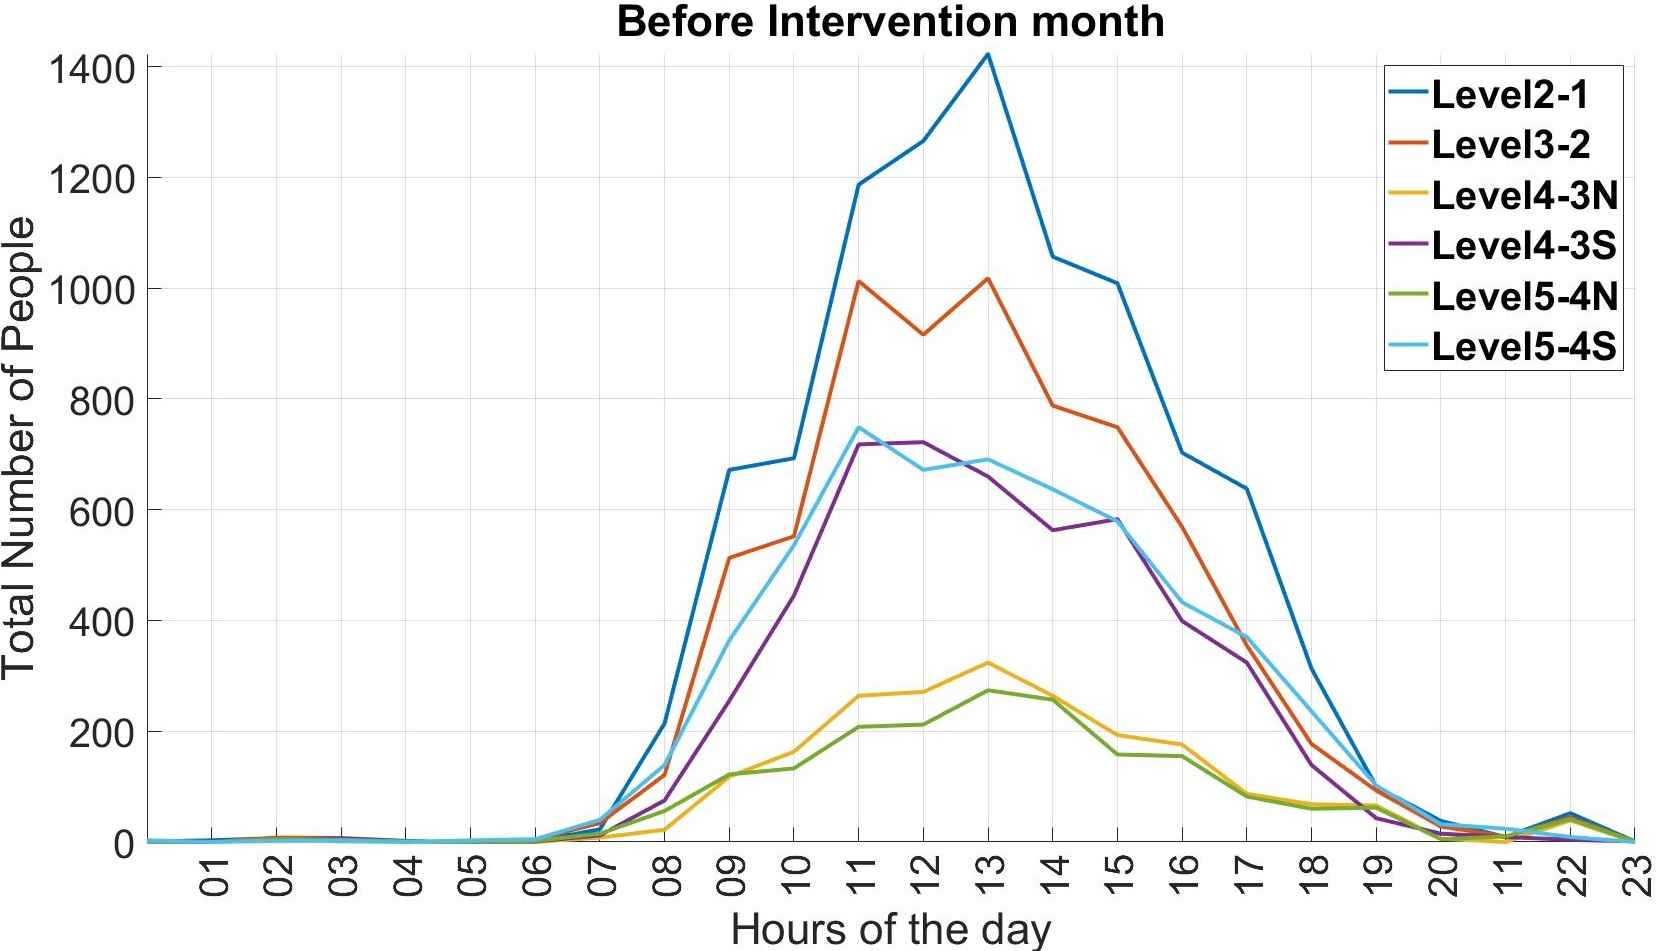
\includegraphics[width=\textwidth]{image/Chapters/Chapter6/before_int.jpg}%\centering
    \end{minipage}
    \begin{minipage}[b]{0.39\textwidth}
    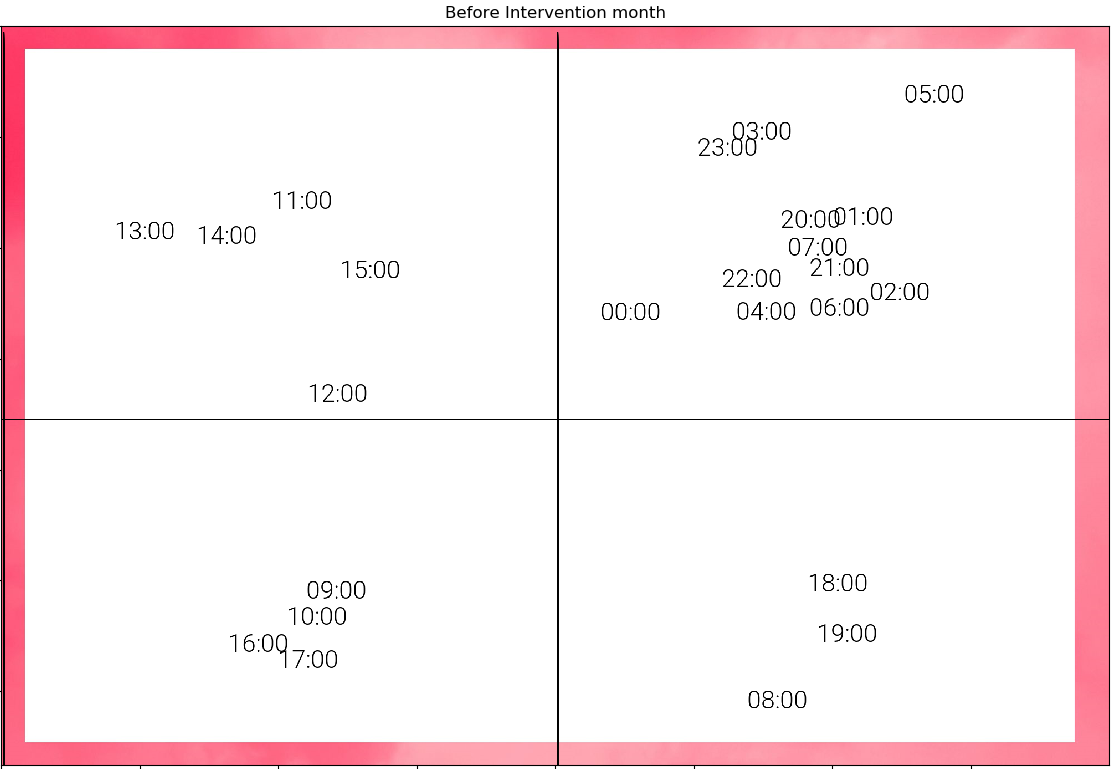
\includegraphics[width=\textwidth]{image/Chapters/Chapter6/timeseriesBefore.png}
    \end{minipage}
    
    \begin{minipage}[b]{0.5\textwidth}
    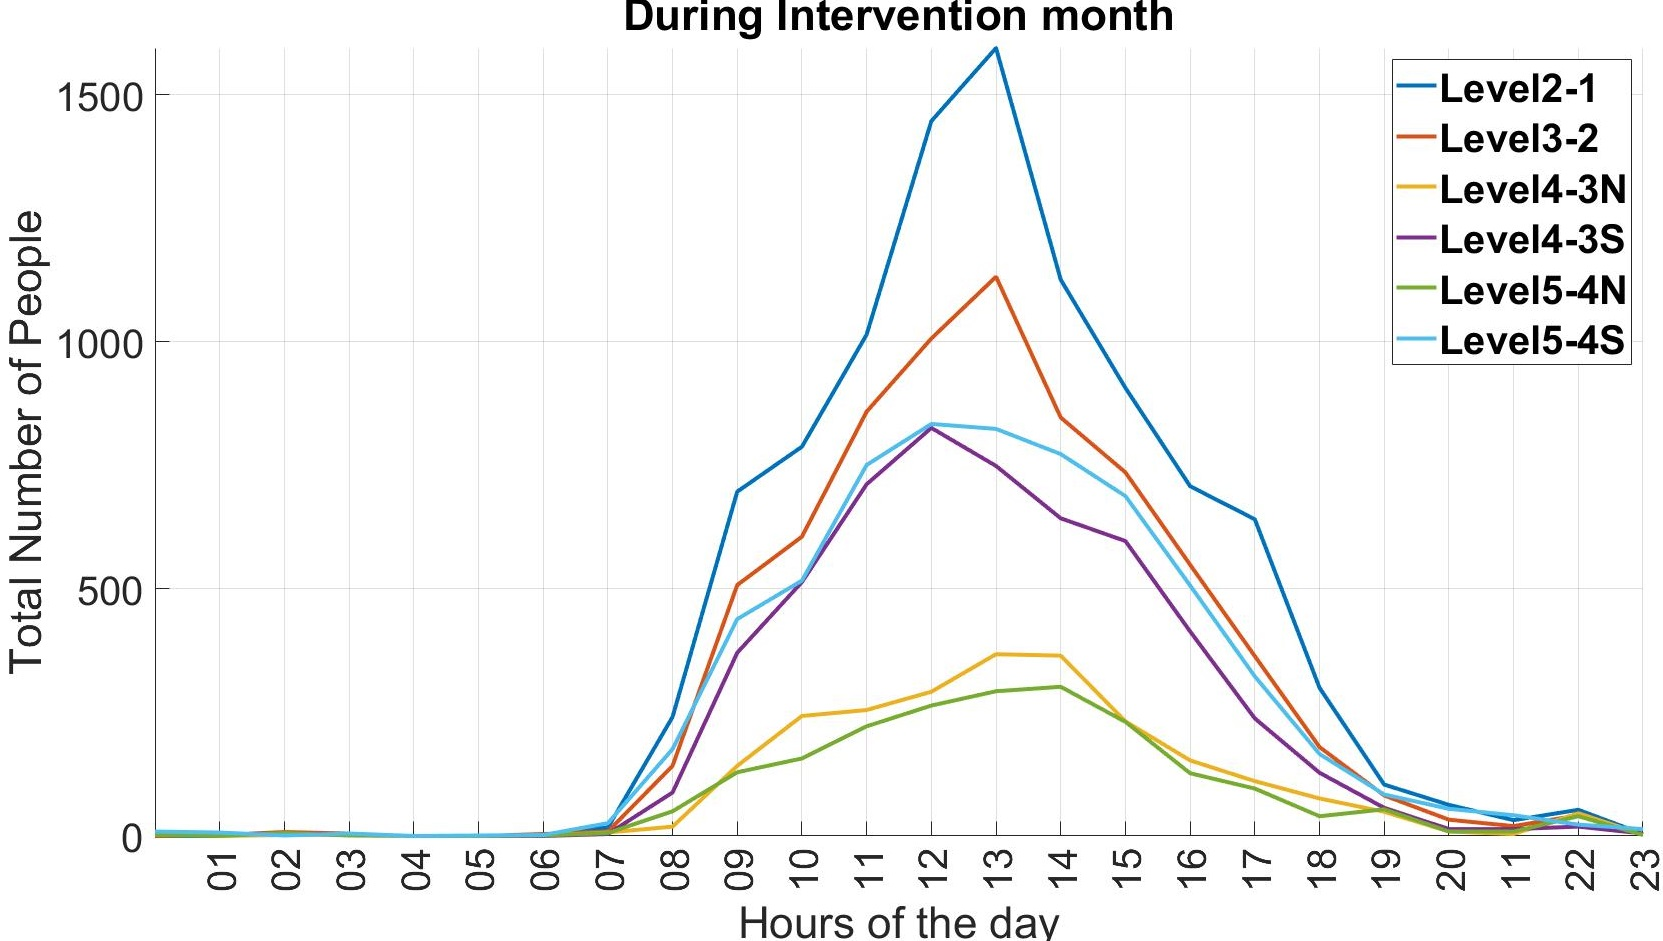
\includegraphics[width=\textwidth]{image/Chapters/Chapter6/during_int.jpg}%\centering
    \end{minipage}
    \begin{minipage}[b]{0.39\textwidth}
    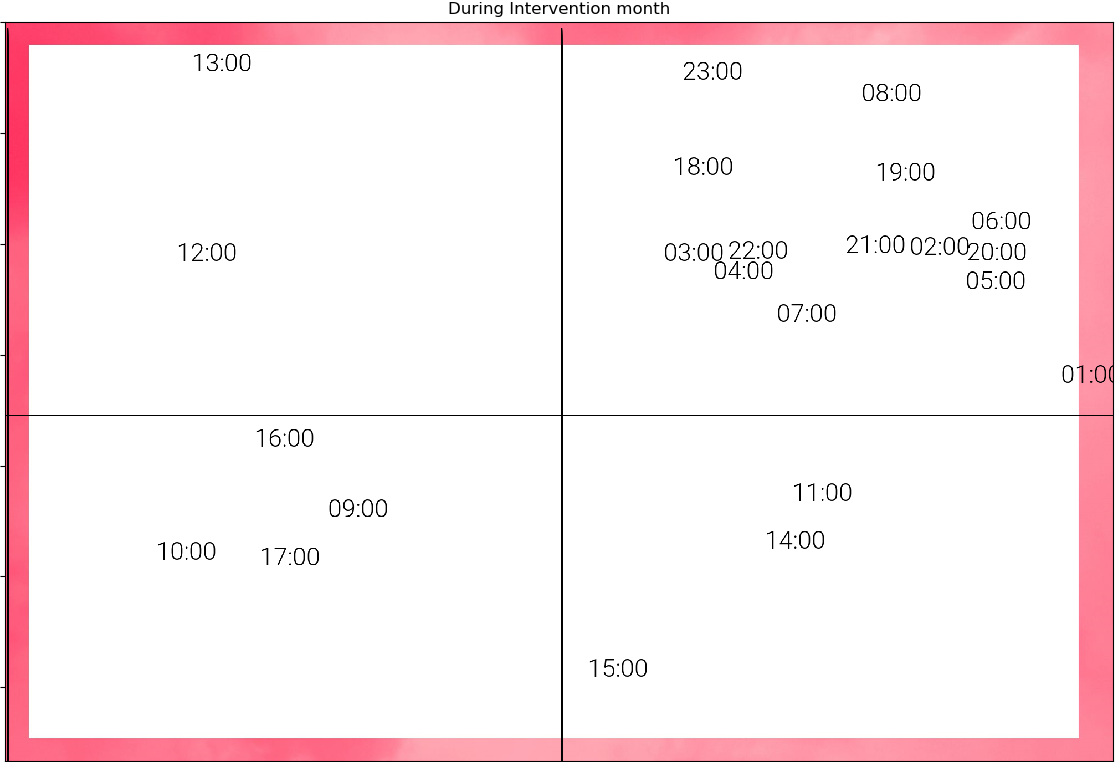
\includegraphics[width=\textwidth]{image/Chapters/Chapter6/timeseriesDuring.png}
    \end{minipage}
    
    \begin{minipage}[b]{0.5\textwidth}
    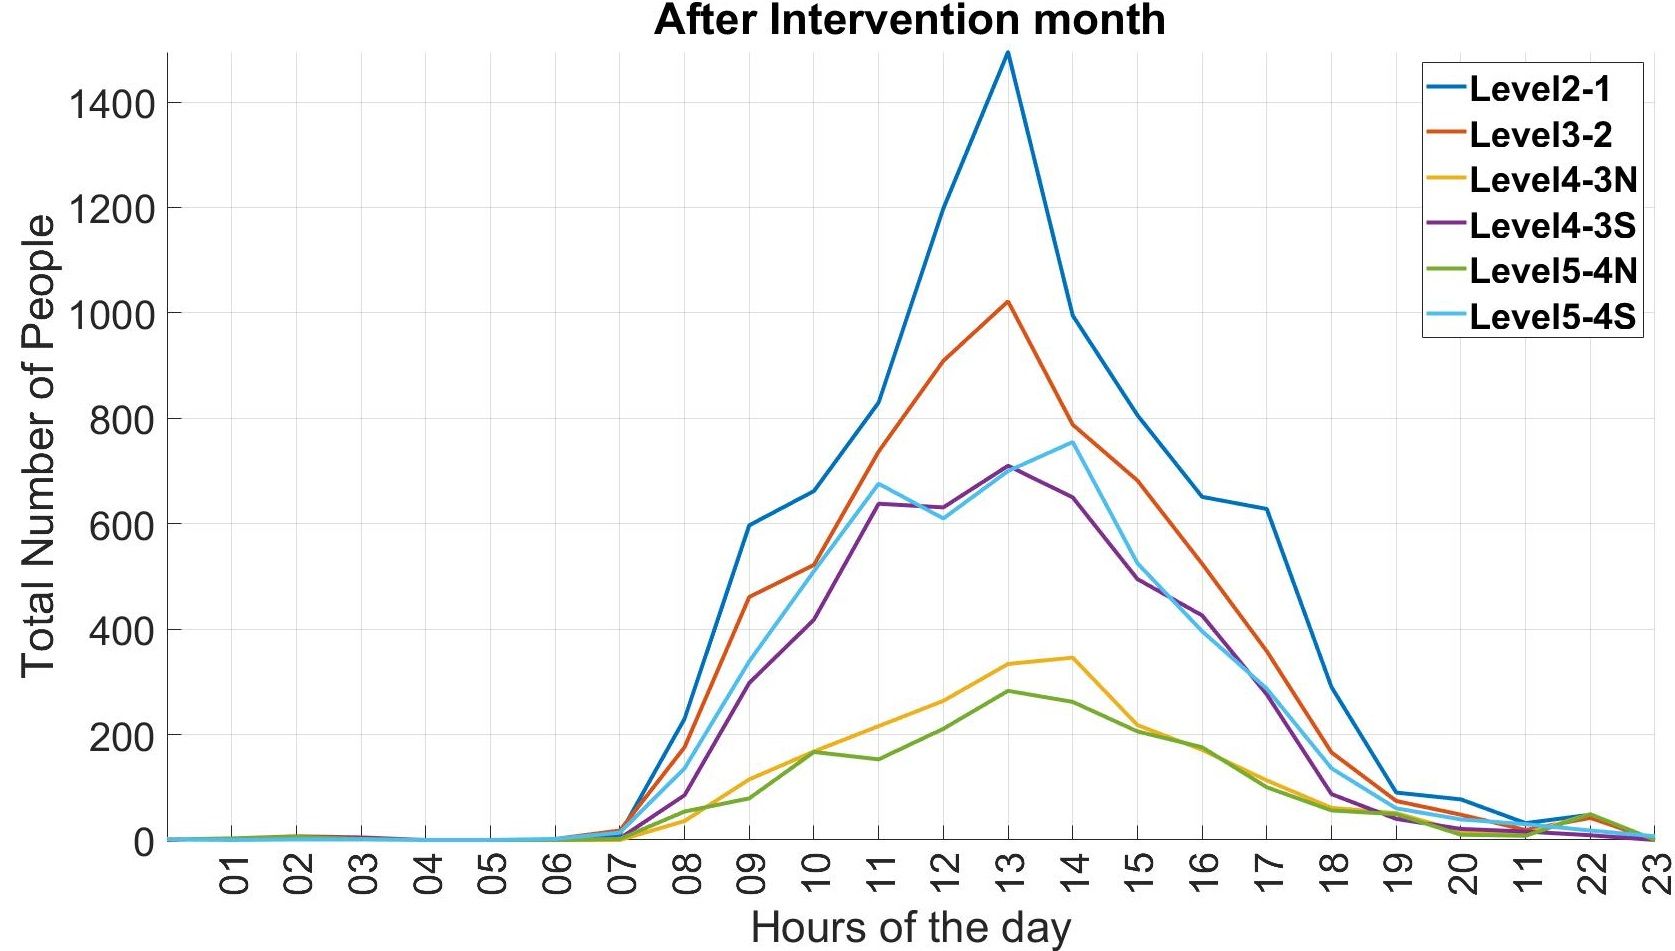
\includegraphics[width=\textwidth]{image/Chapters/Chapter6/after_int.jpg}%\centering
    \end{minipage}
    \begin{minipage}[b]{0.39\textwidth}
    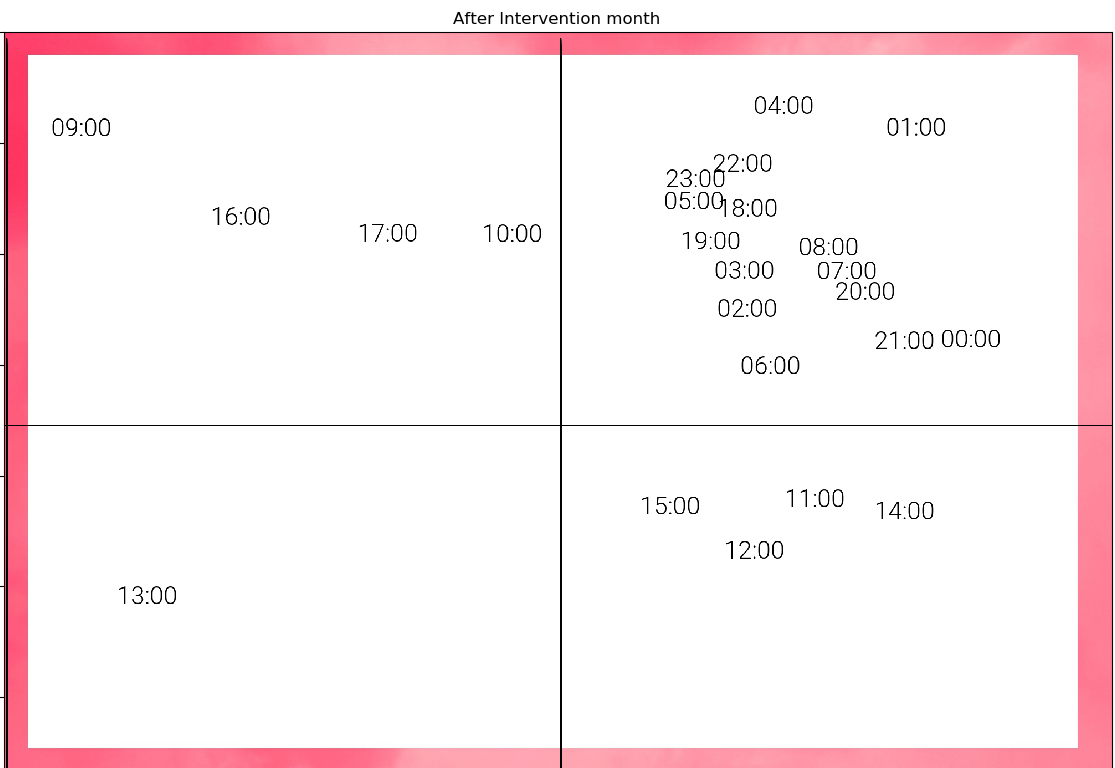
\includegraphics[width=\textwidth]{image/Chapters/Chapter6/timeseriesafter.png}
    \end{minipage}
    \caption{Spatio-temporal patterns during the experiment. \textit{Left}: Hourly stair usage patterns per building level. \textit{Right}: Similar bins of hourly cluster patterns}
    \label{spa1}
\end{figure}

The spatio-temporal patterns found in Figure \ref{spa1} were generated by aggregating the number of people at each level of the building using the three months under analysis. It is clear from the graphs on the left of Figure \ref{spa1} that the Level 2-1 stair were frequently used; meanwhile, levels 4-3 North and 5-4 North were used the least. This could be due to fewer people using the north entrances since the north entrance leads to a low capacity parking lot (refer to Figure \ref{tons} for the Tonsley building layout). These aggregated plots also confirm that the usage peak was around noon. The asymmetry in people count on both sides of the peak is seen in these plots as well. This signifies that consistently people have used the stairs in the afternoon rather than in the morning. 

Finally, Figure \ref{spa1} shows the clustering results that were generated by applying the K-means clustering algorithm on the total number of people found at each hour across all levels. Four bins are used to distinguish the hourly cluster results. The usage peak occurred between 12 pm and 1 pm at Level 2-1 for both during and after intervention months. The stair usage at 11 am, 2 pm, and 3 pm. shows the highest values. During the late evening and early morning hours is expected that the number of people inside the building was low. The last bin consists of the hours with moderate activity seen at the start and end of the workdays. 




%On closer inspection of the experiment log file and Figures \ref{updown} and \ref{3mon}, it was found that on the 10th of May a group of students went up around 12:06 pm and presumably the same group came down at 12:23 pm. This led to an increase in the measured count across many levels, whether this alone accounts for the increase in the accumulated count values for the entire month of intervention can only be confirmed by exploring this observation further which is beyond the scope of this work.





% \begin{figure}[!h]
% \centering
% 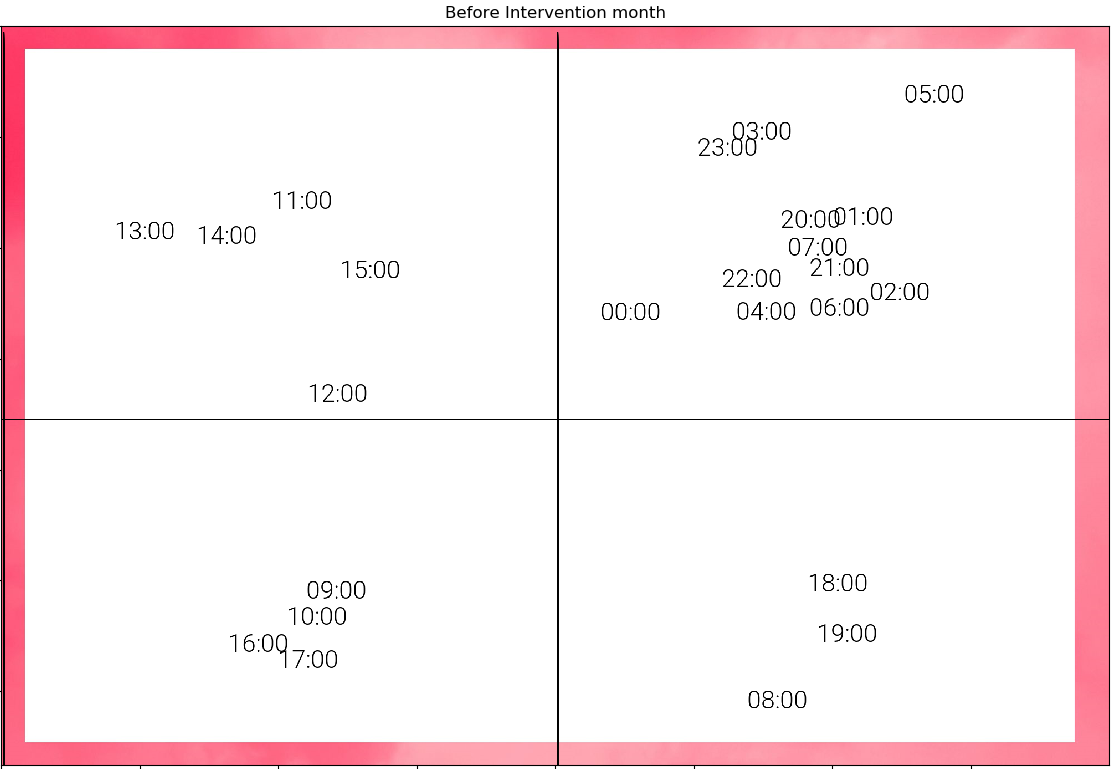
\includegraphics[width=.5\textwidth]{image/Chapters/Chapter6/timeseriesBefore.png}
%     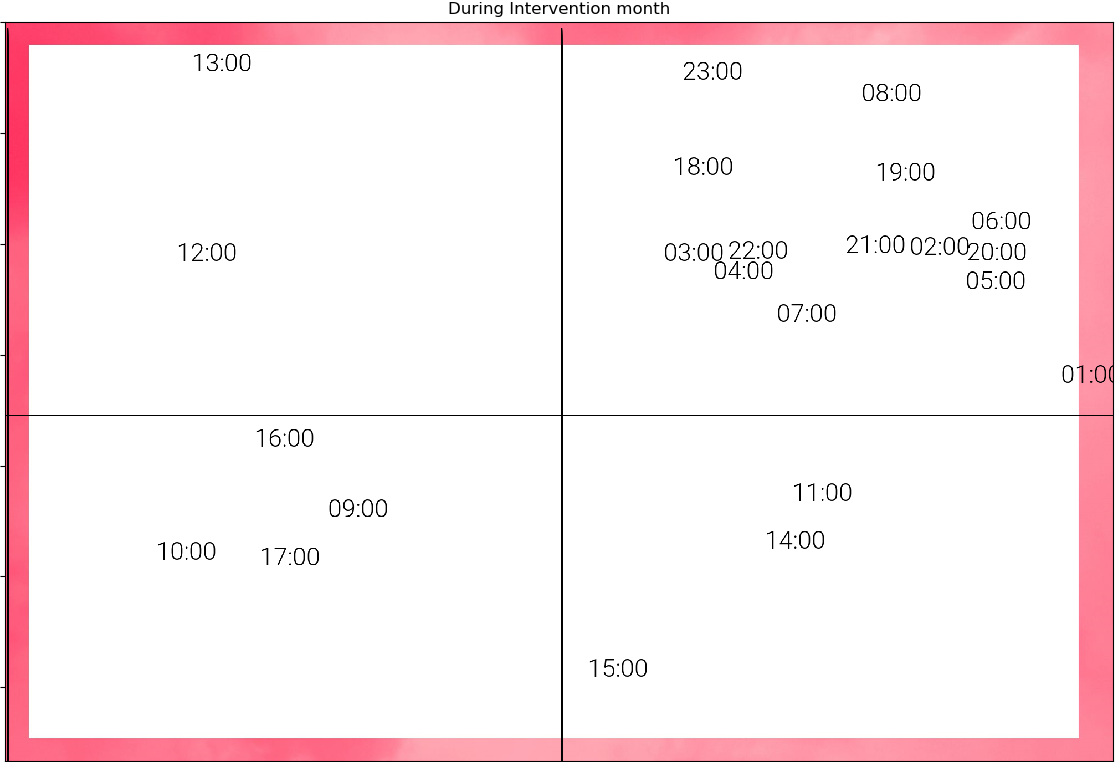
\includegraphics[width=.5\textwidth]{image/Chapters/Chapter6/timeseriesDuring.png}\hfill\centering
%     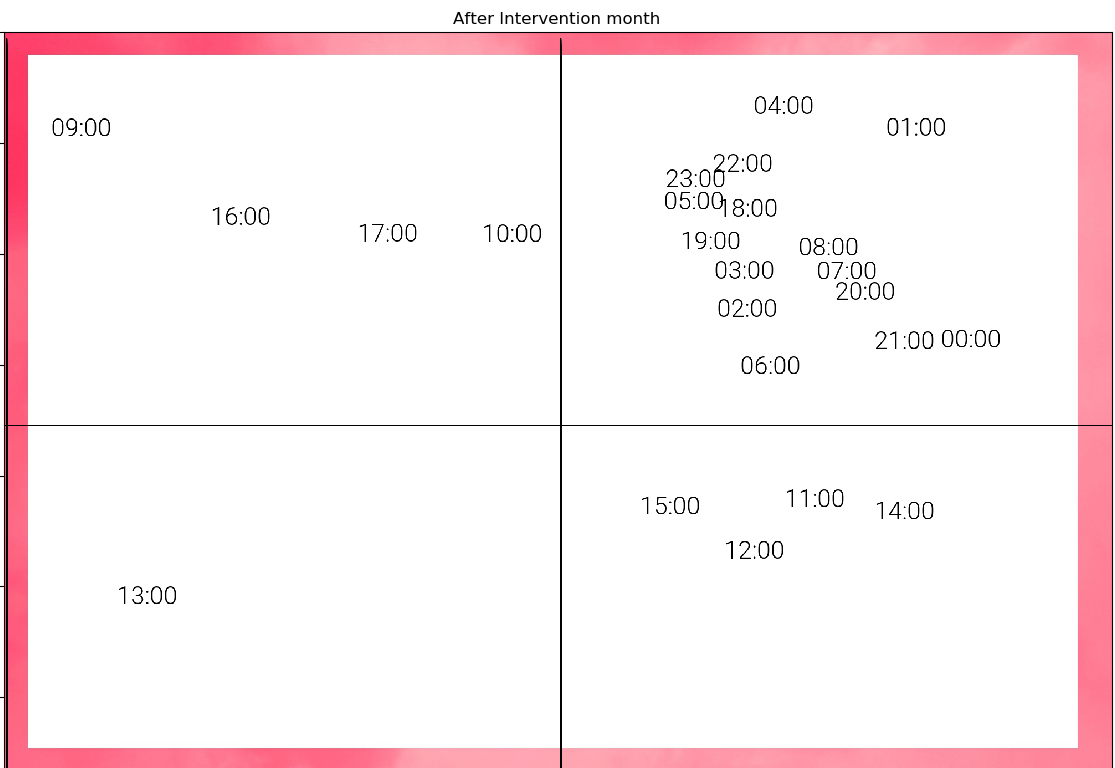
\includegraphics[width=.5\textwidth]{image/Chapters/Chapter6/timeseriesafter.png}
%     \\[\smallskipamount]
% \caption{Hourly clustering of three month of experiment . It shows the similar times per days that have similar pattern. } 
% \label{timegrup}
% \end{figure}


%%%%%%%%%%%%%%%%%%%%%%%%%%%%%%%%%%%%%%%%%%%%%%%%%%%%%%%%%%%%%%%%
%\subsection{M}
%%%%%%%%%%%%%%%%%%%%%%%%%%%%%%%%%%%%%%%%%%%%%%%%%%%%%%%%%%%%%%%%

%The e-counter dataset is an example of spatially distributed measurements that is typically a continuous set of measurements that need to be incrementally interpreted. As the size of the data set increases with time, it soon becomes prohibitively expensive to analyze the entire dataset at a time. Hence to find patterns in the data, data mining techniques like clustering are employed. The e-counter experiment was performed at the Tonsley building in Flinders university to identify if any change in people's behavior was observed due to active educational interventions made over a month's period. In total, more than three months of data were collected during the experiment. YOU ALREADY MENTIONED THIS IN THE IMPLEMENTATION CHAPTER, WHEN YOU DESCRIBED THE EXPERIMENT. THIS CHAPTER IS ONLY ABOUT RESULTS

%As part of the efforts to build a continuous people monitoring and prediction system at the University of New Brunswick \cite{parise2019iot}, several clustering techniques were tried and after comparing a few alternatives the robust unsupervised clustering technique of affinity propagation (AP) was chosen. The standard K-means algorithm is a much lighter algorithm and hence can handle the entire e-counter data set, but the cluster centers produced by K-means do not necessarily coincide with one of the data points that correspond to an actual physical location. Hence due to the difficulty in the physical interpretation of the data, the K-means algorithm was not chosen as the primary tool for data analysis. WHY YOU WOULD TALK ABOUT ALEC'S WORK??? 

%The computer used in this study could only handle data for a week from the e-counter dataset while performing the calculations required for the AP algorithm.  A popular way to analyze large datasets is by treating the data as a continuous stream or analyzing it in batches. The development of the data-streaming affinity propagation algorithm (DSAP) algorithm was motivated by this purpose. Although many stream clustering algorithms have been reported in the literature, but the tuning of the number of hyper-parameters required for each algorithm is not a trivial issue. The simple streaming K-means algorithms, for example, requires an automatic estimation of the number of clusters that can not be easily determined in a changing stream environment. In light of these issues, the DSAP algorithm was preferred for this study. %But, for the sake of completeness and validation, the results from DSAP are compared with those from AP algorithm.   
    
% Figure \ref{oneweek} shows the clusters generated by the AP algorithm for the first week of each of the three months of observation. The first week of the control month before the intervention period was 18 March - 24 March, 29 April - 5 May was the first week of intervention, and the first week after the removal of the educational aids was from 27 May - 2 June. The hyperparameter damping factor chosen for the AP algorithm had the same value of 0.9 for these three weeks. But the other hyperparameter, preference was varied as that depends on the similarity matrix.

% AP clustering algorithm, generally divided the data into clusters with high frequency of low count values and the few instances of high activity for all the three months. The cluster centres in Figure \ref{oneweek} are denoted by large colored circles. The numbers of data points  associated with each cluster is mentioned right next to it. All the branch points of each clusters are represented by points of the same color as the cluster centre. The number of points represented by each cluster help in discerning between the clusters denoting regular behavior from the potentially anomalous clusters that would have remained hidden otherwise. 

% \begin{figure}[!t]
% \centering
% 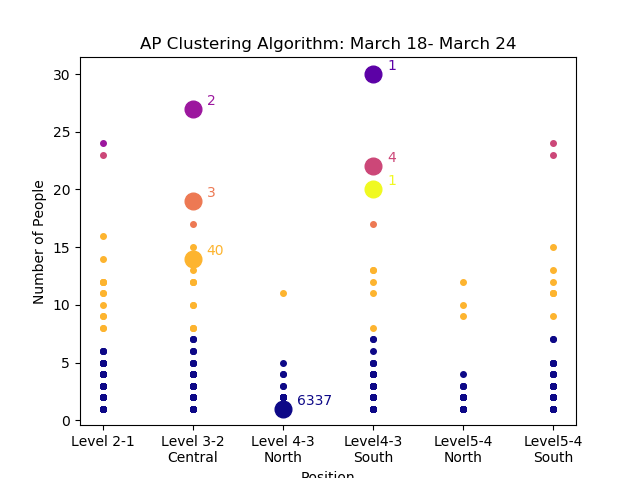
\includegraphics[width=.49\textwidth]{image/Chapters/Chapter6/ApFirstWeekBeforeInt.png}
%     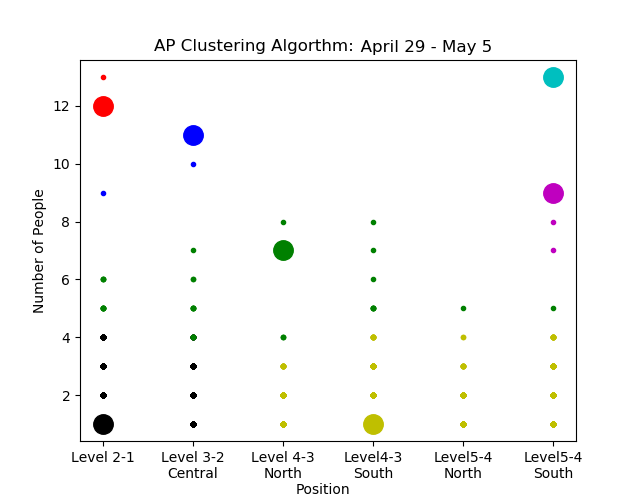
\includegraphics[width=.49\textwidth]{image/Chapters/Chapter6/ApFirstWeekIntervention.png}\hfill\centering
%     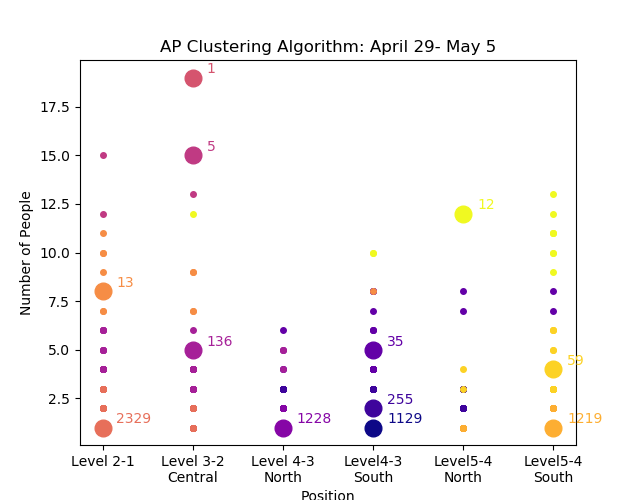
\includegraphics[width=.5\textwidth]{image/Chapters/Chapter6/ApFirstWeekAfterInt.png}
%     \\[\smallskipamount]
% \caption{AP algorithm is applied on e-counter data for first week before, first week during and one week after the intervention month. } 
% \label{oneweek}
% \end{figure}
 
 
% Additional insights into these clusters can be deduced by looking at some statistics for each of the three weeks as shown in Figures. \ref{distbefore} - \ref{distafter}. Each of these three figures shows four plots that show the following features starting clockwise: top-left) hourly stair usage vs measured counts of people passing through, top-right) stair usage by each level vs measured count of people passing through. At the top of this plot the total number of people passing through each level is also provided, bottom right) Histogram of the measurements by each level, and bottom left) The number of instances of number of people recorded by the e-counters.


% Comparing Figures. \ref{oneweek} and \ref{distbefore} for the duration before intervention, we can confirm that the cluster centres with the most numerous points at levels 2-1, 3-2 central, 4-3 south, and 5-4 south with count values of 1-3 are indeed consistent. The high count value of 30 measured around noon as seen in the top left plot was recorded only once (bottom left) at level 4-3 south (top right and Figure. \ref{oneweek}). Other general observations can also be made for this week, for example the highest number of people (top right) and the highest frequency of measurements (bottom right) were made at level 2-1. Curiously a second peak in activity is seen around 15:00-16:00 with count values ranging from 10-15 in the bottom left plot of Figure. \ref{distbefore}. This peak is statistically significant as many of these count values are recorded more than twice going as high as 10 times as seen in the bottom left plot of Figure \ref{distbefore}. This peak was also captured by the AP algorithm as part of the moderate sized cluster geographically placed in the middle at level 4-3 south with count value around 13 as shown in figure \ref{oneweek}.
% \begin{figure}[t]
%     \centering
%       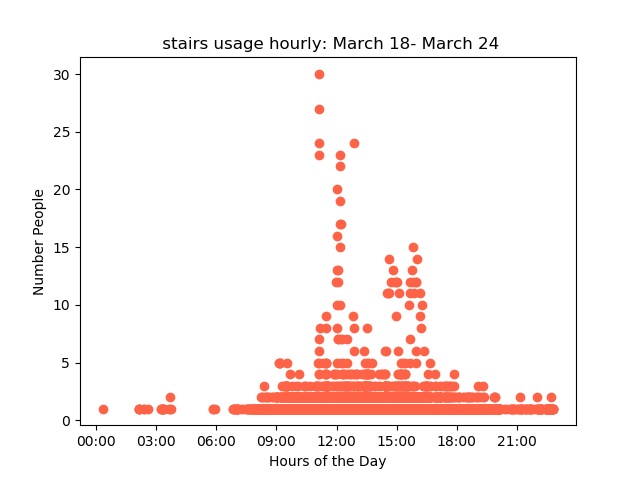
\includegraphics[width=0.42\textwidth]{image/Chapters/Chapter6/oneWeekBeforehourly.png}%\hfill
%     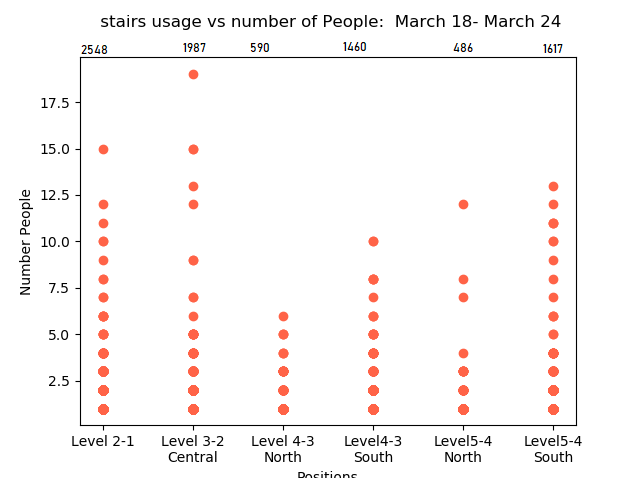
\includegraphics[width=0.42\textwidth]{image/Chapters/Chapter6/PositionCountOneWeekBeforer.png}\hfill
%     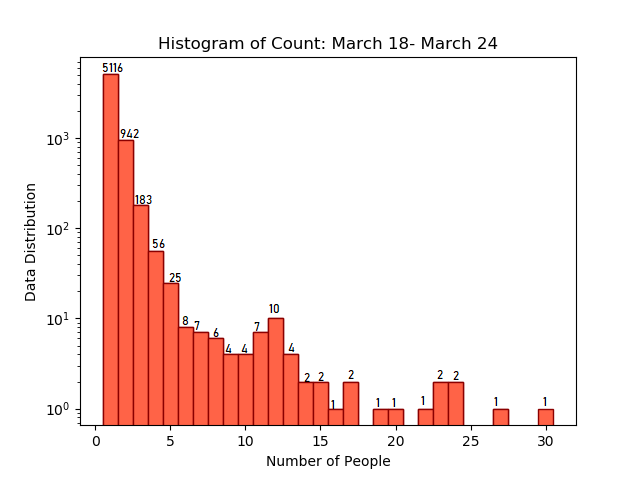
\includegraphics[width=0.42\textwidth]{image/Chapters/Chapter6/oneweekCountDistributonBefore.png}%\hfill 
%     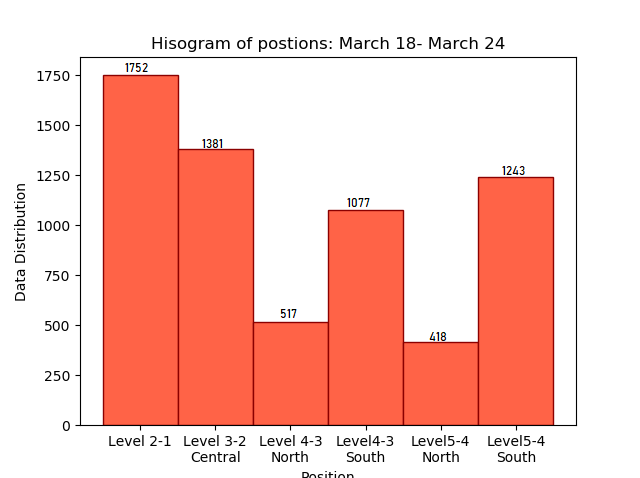
\includegraphics[width=0.42\textwidth]{image/Chapters/Chapter6/oneweekBeforePositionDistributon.png}
%     \caption{One week data distribution. First week before intervention from March 18 - March 24.}
%     \label{distbefore}
% \end{figure}

% \begin{figure}[!h]
%     \centering
   
%     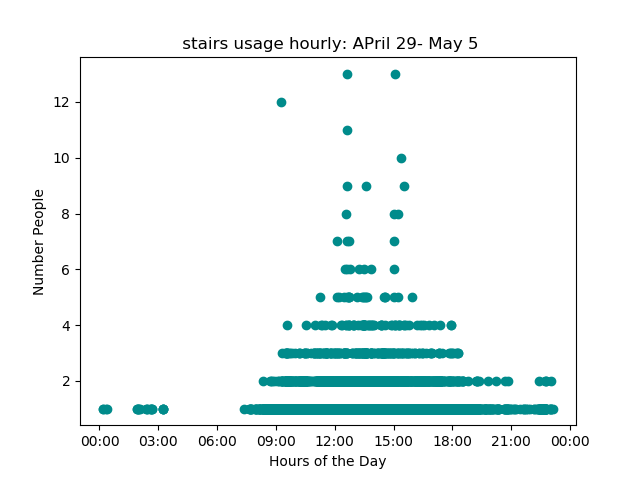
\includegraphics[width=0.42\textwidth]{image/Chapters/Chapter6/oneWeekhourly.png}%\hfill
%     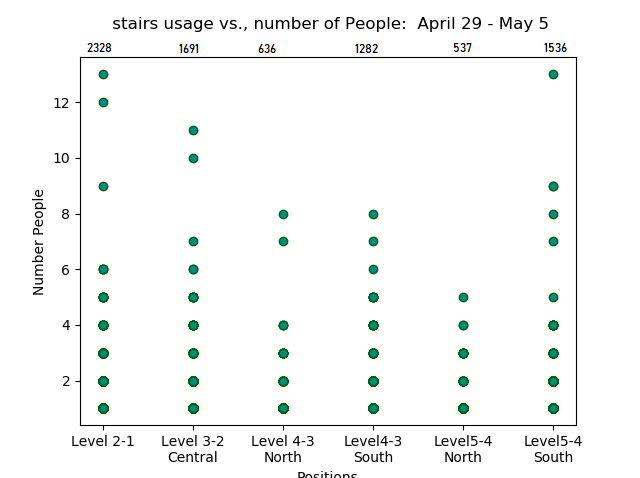
\includegraphics[width=0.42\textwidth]{image/Chapters/Chapter6/PositionCountOneWeek.png}\hfill
%     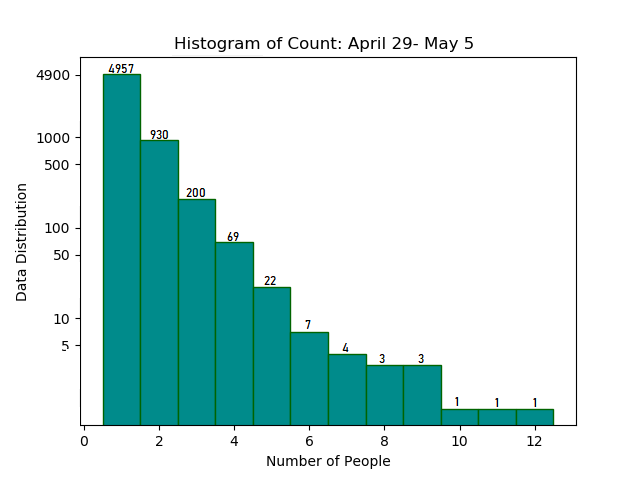
\includegraphics[width=0.42\textwidth]{image/Chapters/Chapter6/oneweekCountDistributon.png}%\hfill 
%     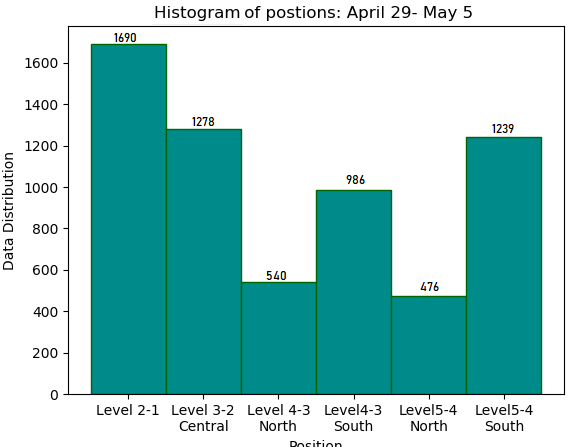
\includegraphics[width=0.42\textwidth]{image/Chapters/Chapter6/oneweekPositionDistributon.png}
%     \caption{One week data distribution. First week of intervention from April 29 -May 5.}
%     \label{distduring}
% \end{figure}

% \begin{figure}[!h]
%     \centering
%       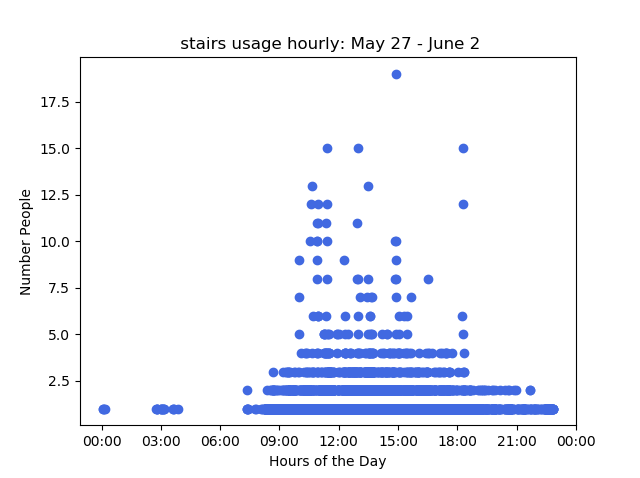
\includegraphics[width=0.45\textwidth]{image/Chapters/Chapter6/oneWeekAfterhourly.png}%\hfill
%     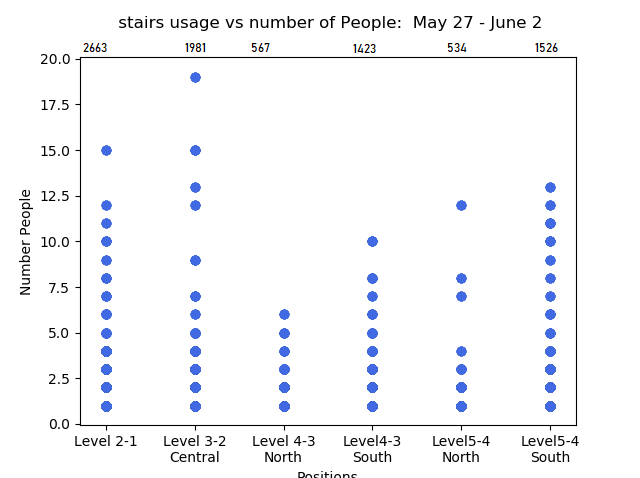
\includegraphics[width=0.45\textwidth]{image/Chapters/Chapter6/PositionCountOneWeekAfter.png}\hfill
%     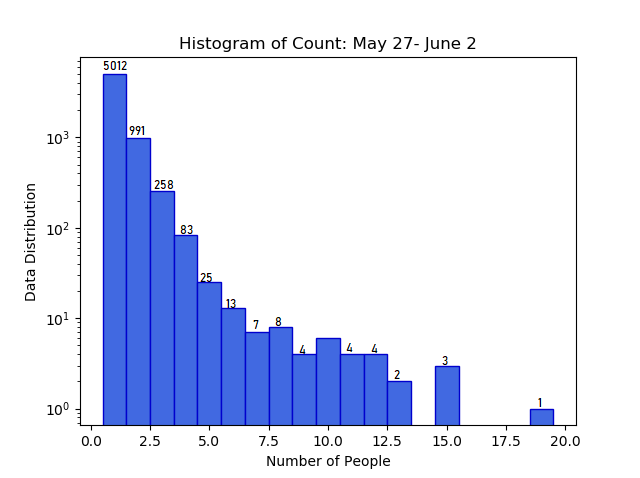
\includegraphics[width=0.47\textwidth]{image/Chapters/Chapter6/oneweekCountDistributonAfter.png}%\hfill 
%     \includegraphics[width=0.47\textwidth]{image/Chapters/Chapter6/oneweekafterPositionDistributon.png}
%     \caption{One week data distribution. First week after intervention from May 27- June 2.}
%     \label{distafter}
% \end{figure}

% The first week of intervention from April 29- May 5 contrary to expectations recorded lower overall activity during the week as shown in Figure \ref{distduring}. This pattern is consistent for almost all the weeks during the intervention month. The month before the intervention period consistently recorded higher activity as compared with the intervention month excluding the anomalous day of May 10th as shown earlier in Figure \ref{3mon}. This week recorded a peak activity around noon and the frequency of recorded counts reduced exponentially from a single count to a high of 12 counts that was recorded only once. The high density clusters corresponding to this week have their cluster centers located at levels 2-1, 3-2 central, 4-3 south, and 5-4 south which are the levels with the highest frequency and number of people. The first week after the end of the intervention period has statistics similar to the intervention week. The frequency of recorded values as shown in the bottom right of Figure \ref{distafter} have similar features like the histogram of the week during intervention. The peak around noon is a lot more spread across hours as shown in the bottom left and top left plots of the Figure.

% The first week after intervention from May 27-June 2 has the same pattern for level 4-3 south and  5-4 south as shown in Figure \ref{distafter}. Additionally, during this week, the number of people moving in level 4-3 north and 5-4 north are almost identical. In this period, the number of people at levels 2-1 and 3-2 was the highest  amongst the three weeks. 
%%%%%%%%%%%%%%%%%%%%%%%%%%%%%%%%%%%%%%%%%%%%%%%%%%%%%%%%%%%%%%%%
\subsection{Micro-cluster Evolution}
%%%%%%%%%%%%%%%%%%%%%%%%%%%%%%%%%%%%%%%%%%%%%%%%%%%%%%%%%%%%%%%%
%DISCUSS FIGURE 6.10
%In order to analyze streaming data or large datasets, batch processing or stream clustering techniques are generally applied. A one hour landmark time window was chosen for the DSAP algorithm to analyze the e-counter dataset. It was found that using a one hour window gave optimum cluster values since this guaranteed that the first time window has enough number of points to initialize the stream clustering process. The hyper-parameters for the AP in the DSAP algorithm are kept fixed at the default values except for the preference value which was set to the median of the similarity matrix. The damping value was kept at 0.9 for the entire experiment.The expiration value was varied from 1 to values corresponding to a week or month depending on the length of the dataset under analysis.% 163. THIS PARAGRAPH TALKS ABOUT IMPLEMENTATION, MOVE THIS CHAPTER IF NEEDED TO THE IMPLEMENTATION.
 
The evolution of micro-clusters was interesting to be analyzed in order to detect any concept drift during the clustering process. In this Section, we discuss the results generated on Wednesday May 1, which were observed between 7 am to 7 pm. Figure \ref{APhourly} shows the centroids of the micro-clusters and their respective data points that are connected using straight lines. The one-hour expiration time was chosen to ensure that only the data points within the one-hour window were used for finding clusters. 

The changes in stair usage across all levels can be clearly seen in Figure \ref{APhourly}. The micro-clusters show an increase in activity starting around 9-11 am. At the peak around noon, the micro-clusters become more dense occurring at different levels of the building. As the day progresses, the number of micro-clusters gradually decreases. These generated patterns were observed throughout the experiment, demonstrating the potential of using the DSAP approach for finding and tracking meaningful micro-clusters over space and time. The strength of DSAP lies in its ability to continuously find micro-clusters by responding quickly to any changes in the stream data.

% \begin{figure}[!h]
%     \centering
   
%     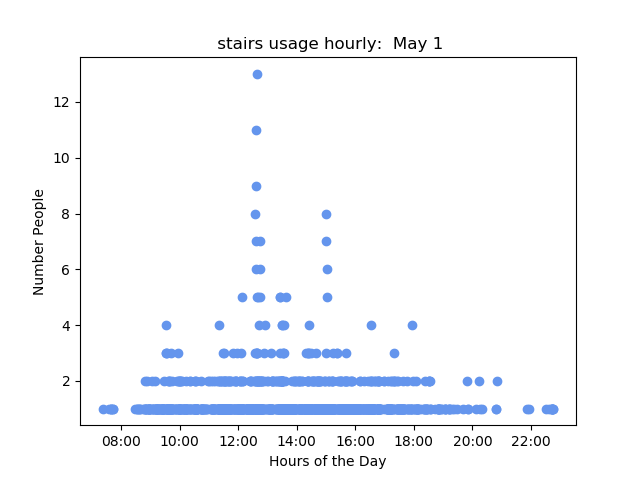
\includegraphics[width=0.5\textwidth]{image/Chapters/Chapter6/onedayhourMay1.png}\hfill
%     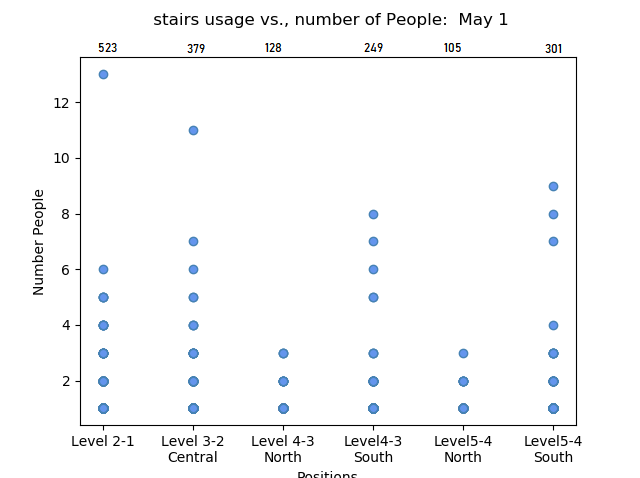
\includegraphics[width=0.5\textwidth]{image/Chapters/Chapter6/1day1monday1InterventionD.png}\hfill
%     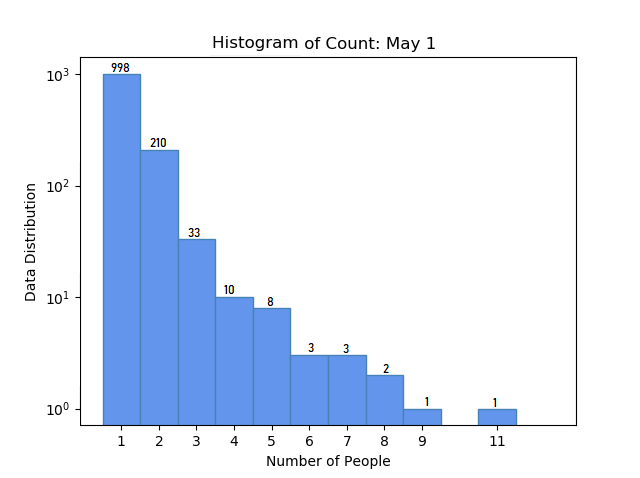
\includegraphics[width=0.5\textwidth]{image/Chapters/Chapter6/oneweekCountApril.png}\hfill 
%     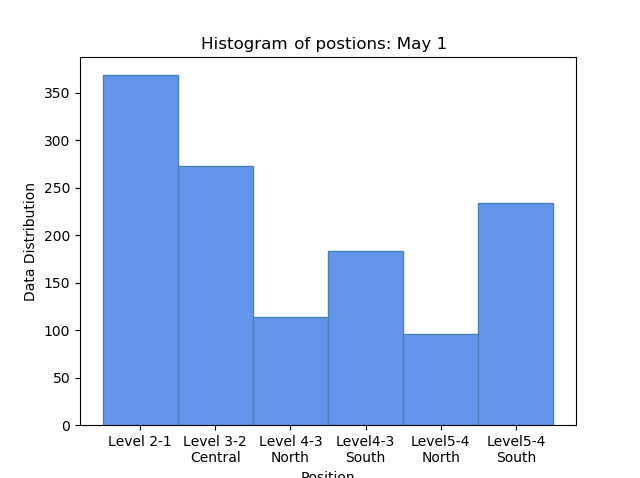
\includegraphics[width=0.5\textwidth]{image/Chapters/Chapter6/oneweek(Monday)Hist.png}
%     \caption{One day data distribution. First Wednesday of intervention: May 1. Top left- The total count of people at all the levels during the entire day starting at 7 a.m. Top right- The measured count of people at each level for the day. Bottom left- Histogram of the people count registered at all levels. Bottom right- Histogram of the measurements made at each level for the day }
%     \label{1daystat}
% \end{figure}


%This day follows the overall pattern of stair usage as shown in the top-left panel of the Figure \ref{1daystat} which matches with the trends seen earlier in the aggregate plots \ref{spa2}. The accumulated number of people passing through a particular level is mentioned at the top of the panel shown in the top right of Figure \ref{1daystat}. This figure also shows the spatial distribution of measurements for the day. It should be noticed that levels 3-2 and 5-4 have similar aggregated numbers, but it seems like the contribution comes from a higher percentage of high value counts for level 5-4.

%The bottom left panel of Figure \ref{1daystat} clearly shows that the maximum number of records measures only one person. Note that the scale of the y-axis is logarithmic and the number of records with higher count values reduces exponentially. The position histogram for the day is shown in the bottom-right of the same figure. On this day too the highest number of counts were observed on level 2-1 while both the north-side levels (4-3 North and 5-4 North) record the least activity that is at least three times lower than those of level 2-1. 


\begin{figure}[htp]
%\centering
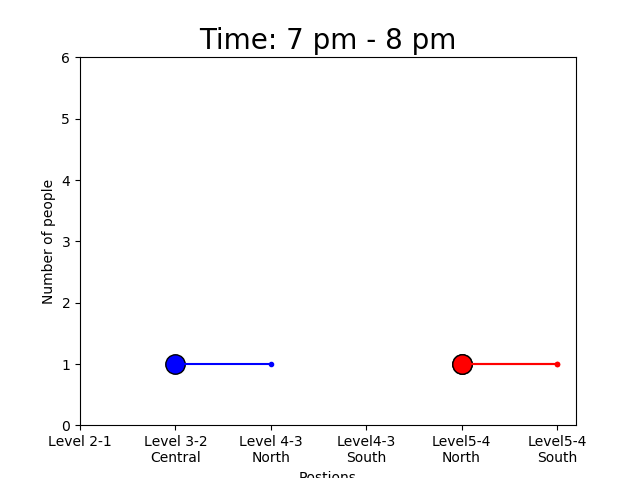
\includegraphics[width=.33\textwidth]{image/Chapters/Chapter6/7.png}%\quad
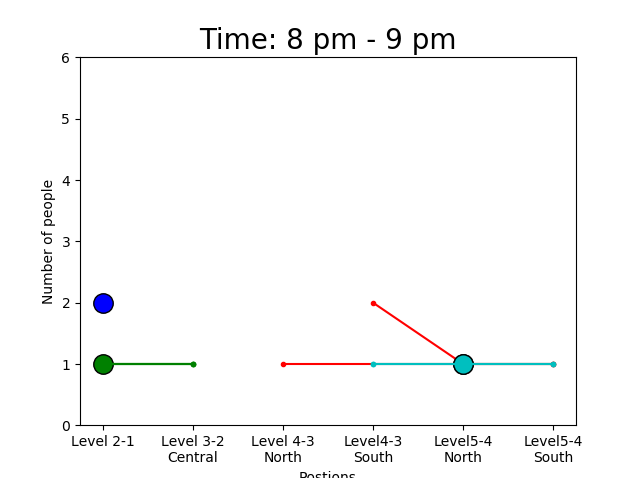
\includegraphics[width=.33\textwidth]{image/Chapters/Chapter6/8.png}%\quad
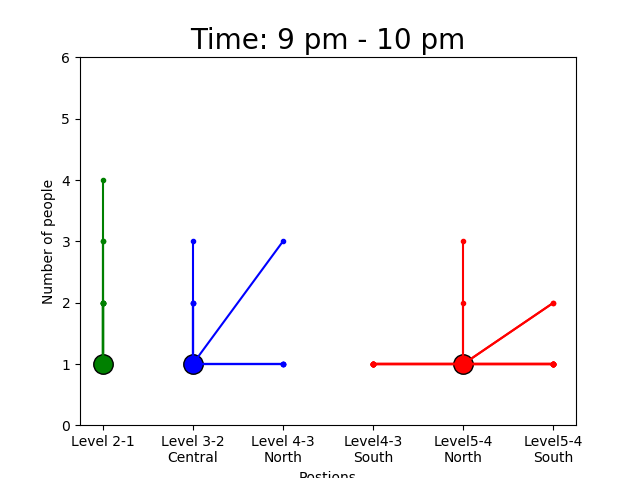
\includegraphics[width=.33\textwidth]{image/Chapters/Chapter6/9.png}

% \medskip

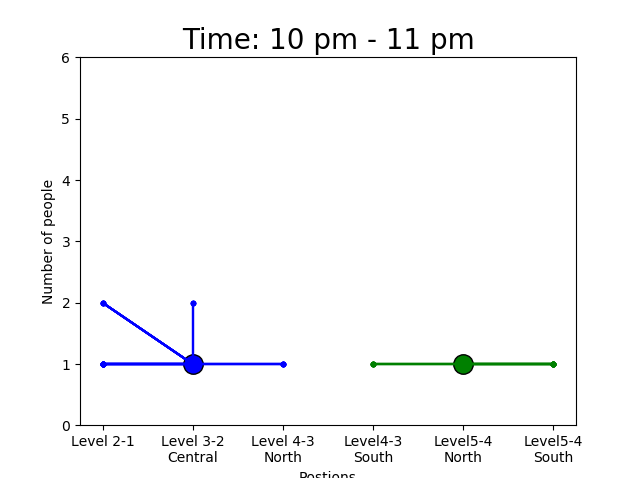
\includegraphics[width=.33\textwidth]{image/Chapters/Chapter6/10.png}%\quad
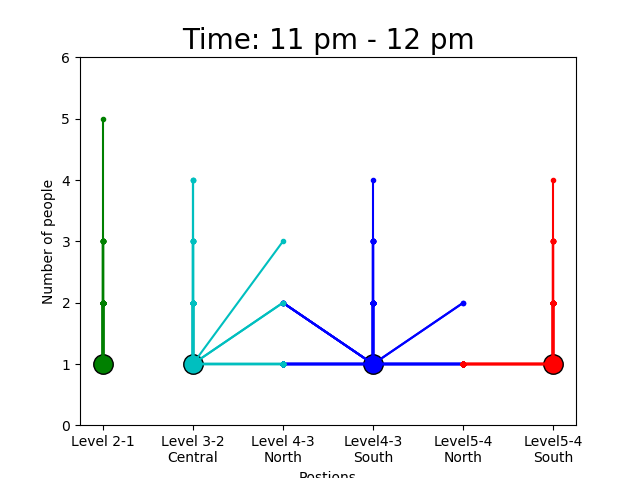
\includegraphics[width=.33\textwidth]{image/Chapters/Chapter6/11.png}%\quad
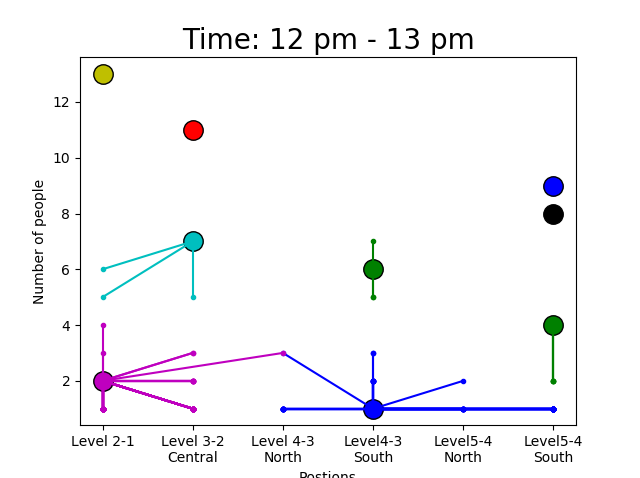
\includegraphics[width=.33\textwidth]{image/Chapters/Chapter6/12.png}

% \medskip

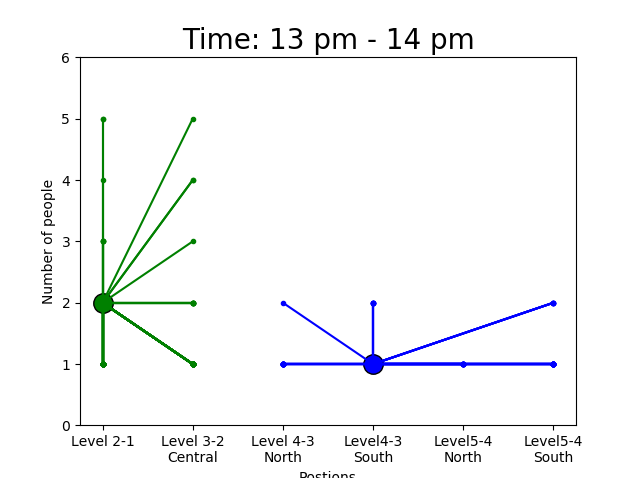
\includegraphics[width=.33\textwidth]{image/Chapters/Chapter6/13.png}%\quad
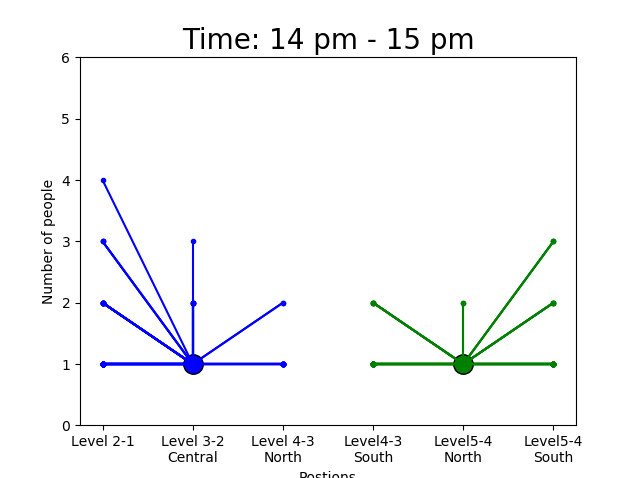
\includegraphics[width=.33\textwidth]{image/Chapters/Chapter6/14.png}%\quad
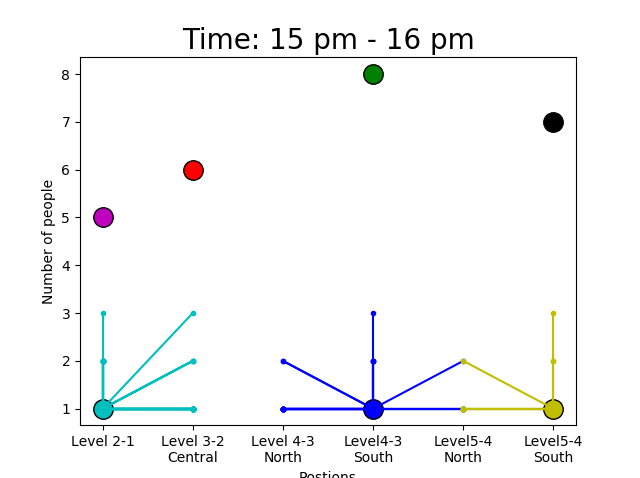
\includegraphics[width=.33\textwidth]{image/Chapters/Chapter6/15.png}
% \medskip

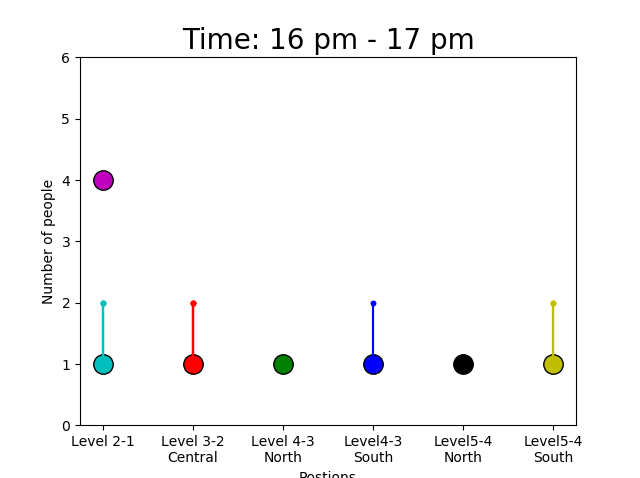
\includegraphics[width=.33\textwidth]{image/Chapters/Chapter6/16.png}%\quad
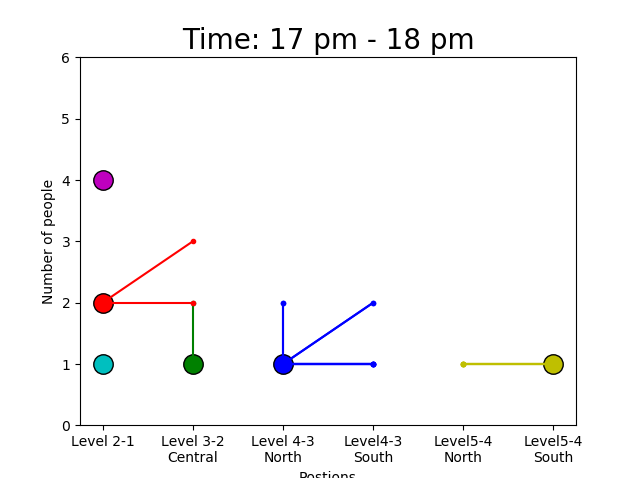
\includegraphics[width=.33\textwidth]{image/Chapters/Chapter6/17.png}%\quad
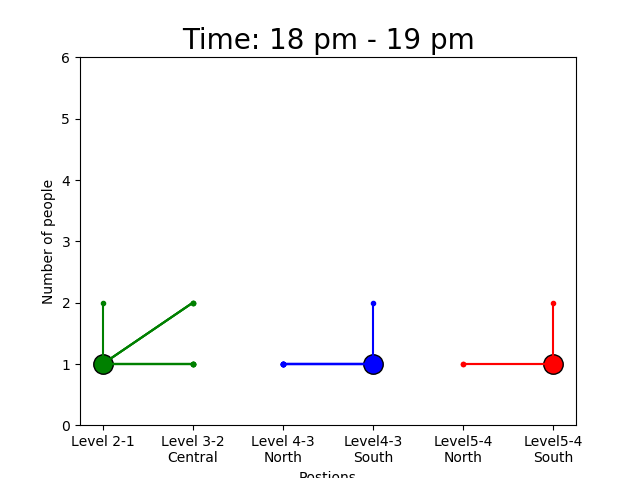
\includegraphics[width=.33\textwidth]{image/Chapters/Chapter6/18.png}

\caption{The evolution of micro-clusters between 7 am to 7 pm on Wednesday May 1, 2019} %Affinity propagation clustering Algorithm with the number of people at different stairs for each hour with landmark time window , first week of intervention month. Early Hours Clusters; Mid-Morning; Lunch-time Hourly; Afternoon time}
\label{APhourly}
\end{figure}

\subsection{Generated Micro and Macro-clusters}

The DSAP clustering results are presented by visualizing all the centroids of the micro-clusters as blue circles while the centroids of the macro-clusters are represented as red crosses. The data points are visualized as black dots. The numbers of data points associated with each micro-cluster are mentioned right next to it. Searching for meaningful clusters has been achieved by evaluating weekly and monthly patterns.


\textbf{Weekly Patterns}

The first week of each of the three months under study was selected to interpret the clustering results. The first week of 18 March - 24 March before the intervention, the first week of 29 April - 5 May during the intervention, and the first week after the removal of the educational aids was from 27 May - 2 June. The selected expiration time equals to 168 was used for generating weekly patterns that are summarized in Table \ref{mactab}. Five macro-clusters have been found for each week, having a variety of density values ranging from 11 up to 4520. This overall trend of high-density clusters with low counts was consistently present in data. It is also interesting to point out that the same macro-cluster (4,1) has happened during the three weeks of the analysis, but having a different number of micro-clusters containing a large number of data points. 

\begin{table}[t]
\small
\centering
\caption{Weekly Clustering Statistics}
\label{mactab}
\begin{tabular}{clcc}
\hline
\textbf{Macro-Cluster} & \textbf{\begin{tabular}[c]{@{}l@{}}Coordinates\\ in the Plot\end{tabular}} & \textbf{\begin{tabular}[c]{@{}c@{}}Number of \\ Micro-Cluster\end{tabular}} & \textbf{\begin{tabular}[c]{@{}c@{}}Total Number of \\ Data Points \end{tabular}} \\ \hline\midrule
\multicolumn{4}{c}{\cellcolor[HTML]{ECF4FF}\textbf{First Week Before Intervention (March 18 - March 24)}}                                                                                                                                                                   \\ \hline
\textbf{1}             & (1,1)                                                                      & 1                                                                           & 1603                                                                                    \\ \hline
\textbf{2}             & (1,9)                                                                      & 3                                                                           & 64                                                                                      \\ \hline
\textbf{3}             & (4,1)                                                                      & 6                                                                           & 4520                                                                                    \\ \hline
\textbf{4}             & (4,22)                                                                     & 2                                                                           & 13                                                                                      \\ \hline
\textbf{5}             & (6,5)                                                                      & 3                                                                           & 82                                                                                      \\ \hline
\multicolumn{4}{c}{\cellcolor[HTML]{ECF4FF}\textbf{First Week During Intervention (April 29 - May 5)}}                                                                                                                                                                      \\ \hline
\textbf{1}             & (1,5)                                                                      & 3                                                                           & 109                                                                                     \\ \hline
\textbf{2}             & (2,1)                                                                      & 5                                                                           & 4388                                                                                    \\ \hline
\textbf{3}             & (2,11)                                                                     & 3                                                                           & 6                                                                                       \\ \hline
\textbf{4}             & (4,1)                                                                      & 1                                                                           & 921                                                                                     \\ \hline
\textbf{5}             & (6,1)                                                                      & 3                                                                           & 1664                                                                                    \\ \hline
\multicolumn{4}{c}{\cellcolor[HTML]{ECF4FF}\textbf{First Week After Intervention (May 27 - June 2)}}                                                                                                                                                                        \\ \hline
\textbf{1}             & (1,3)                                                                      & 4                                                                           & 3269                                                                                    \\ \hline
\textbf{2}             & (2,15)                                                                     & 3                                                                           & 11                                                                                      \\ \hline
\textbf{3}             & (4,1)                                                                      & 1                                                                           & 1810                                                                                    \\ \hline
\textbf{4}             & (4,8)                                                                      & 4                                                                           & 36                                                                                      \\ \hline
\textbf{5}             & (6,3)                                                                      & 4                                                                           & 1207                                                                                    \\ \hline\midrule
\end{tabular}
\end{table}

Figure \ref{dsap3week} illustrate the occurrence of the weekly patterns at different levels of the building, revealing that the intervention campaign had a positive impact on people taking the stairs between level 3-2 and level 4-3 south. In contrast, the campaign has also shown to have a weak impact in changing the behaviour of people when taking the stairs between level 4-3 and level 5-4. Finally, the intervention campaign has not increased the usage of stairs between level 2-1. No anomalous clusters were found in these results. 


\begin{figure}[!t]
    \centering
    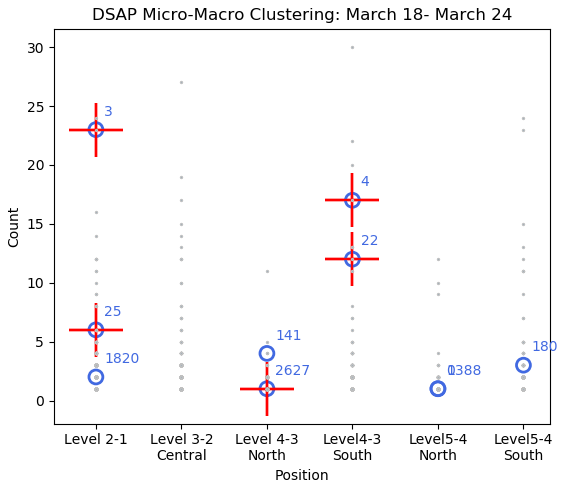
\includegraphics[width=.47\textwidth]{image/Chapters/Chapter6/beforeInte1week.png}
    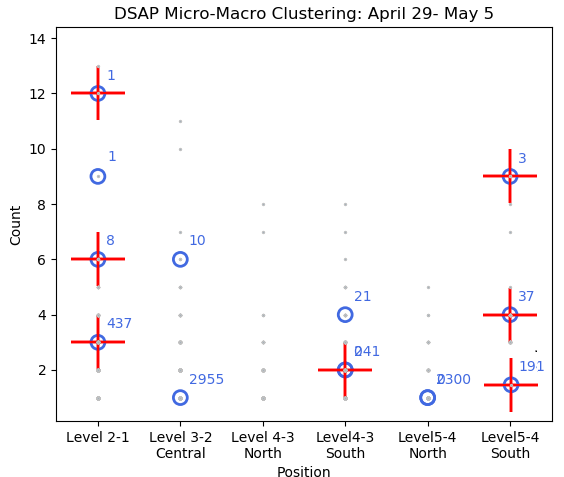
\includegraphics[width=.5\textwidth]{image/Chapters/Chapter6/duringInte1week.png}
    \includegraphics[width=.5\textwidth]{image/Chapters/Chapter6/afterInte1week.png}
    \caption{Clustering results for the first week before, during, and after the intervention campaign}
    \label{dsap3week}
\end{figure}



%\todo[inline]{Figure \ref{oneweek} shows the clusters generated by the AP algorithm for the first week of each of the three months of observation. The first week of the control month before the intervention period was 18 March - 24 March, 29 April - 5 May was the first week of intervention, and the first week after the removal of the educational aids was from 27 May - 2 June. COMPARISON BETWEEN BASELINE AP MODEL?} L

%\todo[inline]{The hyperparameter damping factor chosen for the AP algorithm had the same value of 0.9 for these three weeks. But the other hyperparameter, preference was varied as that depends on the similarity matrix. THIS BELONGS TO THE IMPLEMENTATION CHAPTER, havent you mentioned already in the implementation chapter???}

%\todo[inline]{(The expiration time defined as the time duration within which a data point stays relevant for computing the micro-clusters was set to .

\textbf{Monthly Patterns}

The expiration time value of 670 was used to compute the monthly patterns as shown in Table \ref{monthmacro}. For the first month, eight macro-clusters, during the intervention, twelve and after intervention ten macro-clusters have been found. The total number of data points associated to micro-clusters are varied between 1 up to 13460. Interestingly, all macro-clusters for these three months are for levels 2-1, 3-2, 4-3 south and 5-4 south.  


Figure \ref{dsap3mon} depicted the monthly pattern generated by the DSAP clustering algorithm in this building during the three months of the experiment. These results show that for the entire month of intervention, more clusters appeared. 


\todo[inline]{Nasrin: can we have a table with the clustering statistics for the monthly clusters???? Is that something easy to do?? or it is time consuming???}

\todo[inline]{I was not able to find any explanation of Figure 6.7. If you find it, can you copy it here. Otherwise, I will wrote a paragraph about it}




\begin{table}
\centering
\small
\caption{Monthly Clustering Statistics}
\label{monthmacro}
\begin{tabular}{cccc}
\hline
\textbf{Macro-Clusters} & \textbf{\begin{tabular}[c]{@{}c@{}}Coordinates\\ in the Plot\end{tabular}} & \textbf{\begin{tabular}[c]{@{}c@{}}Number of\\ Micro-Clusters\end{tabular}} & \textbf{\begin{tabular}[c]{@{}c@{}}Total Number Of\\ Data Points\end{tabular}} \\ \hline\midrule
\multicolumn{4}{c}{\cellcolor[HTML]{ECF4FF}\textbf{First Week Before Intervention (March 18 - April 14)}}                                                                                                                                                           \\ \hline
\textbf{1}              & (1,1)                                                                      & 1                                                                           & 6251                                                                           \\ \hline
\textbf{2}              & (1,6)                                                                      & 1                                                                           & 88                                                                             \\ \hline
\textbf{3}              & (2,1)                                                                      & 1                                                                           & 6471                                                                           \\ \hline
\textbf{4}              & (2,31)                                                                     & 2                                                                           & 3                                                                              \\ \hline
\textbf{5}              & (4,12)                                                                     & 1                                                                           & 53                                                                             \\ \hline
\textbf{6}              & (4,17)                                                                     & 1                                                                           & 22                                                                             \\ \hline
\textbf{7}              & (6,3)                                                                      & 2                                                                           & 6922                                                                           \\ \hline
\textbf{8}              & (6,23)                                                                     & 2                                                                           & 16                                                                             \\ \hline
\multicolumn{4}{c}{\cellcolor[HTML]{ECF4FF}\textbf{First Week During Intervention (April 29 - May 26)}}                                                                                                                                                             \\ \hline
\textbf{1}              & (1,5)                                                                      & 1                                                                           & 183                                                                            \\ \hline
\textbf{2}              & (1,13)                                                                     & 1                                                                           & 8                                                                              \\ \hline
\textbf{3}              & (1,23)                                                                     & 1                                                                           & 1                                                                              \\ \hline
\textbf{4}              & (1,30)                                                                     & 1                                                                           & 2                                                                              \\ \hline
\textbf{5}              & (2,3)                                                                      & 2                                                                           & 13460                                                                          \\ \hline
\textbf{6}              & (2,11)                                                                     & 1                                                                           & 16                                                                             \\ \hline
\textbf{7}              & (2,16)                                                                     & 1                                                                           & 5                                                                              \\ \hline
\textbf{8}              & (4,2)                                                                      & 3                                                                           & 4068                                                                           \\ \hline
\textbf{9}              & (4,7)                                                                      & 1                                                                           & 24                                                                             \\ \hline
\textbf{10}             & (6,5)                                                                      & 2                                                                           & 816                                                                            \\ \hline
\textbf{11}             & (6,13)                                                                     & 1                                                                           & 9                                                                              \\ \hline
\textbf{12}             & (6,22)                                                                     & 1                                                                           & 1                                                                              \\ \hline
\multicolumn{4}{c}{\cellcolor[HTML]{ECF4FF}\textbf{First Week After Intervention (May 27 - June 23)}}                                                                                                                                                               \\ \hline
\textbf{1}              & (1,1)                                                                      & 2                                                                           & 10846                                                                          \\ \hline
\textbf{2}              & (1,11)                                                                     & 1                                                                           & 8                                                                              \\ \hline
\textbf{3}              & (2,7)                                                                      & 3                                                                           & 144                                                                            \\ \hline
\textbf{4}              & (2,15)                                                                     & 1                                                                           & 8                                                                              \\ \hline
\textbf{5}              & (2,19)                                                                     & 1                                                                           & 3                                                                              \\ \hline
\textbf{6}              & (4,1)                                                                      & 1                                                                           & 6819                                                                           \\ \hline
\textbf{7}              & (6,2)                                                                      & 4                                                                           & 4188                                                                           \\ \hline
\textbf{8}              & (6,6)                                                                      & 1                                                                           & 19                                                                             \\ \hline
\textbf{9}              & (6,11)                                                                     & 1                                                                           & 8                                                                              \\ \hline
\textbf{10}             & (6,18)                                                                     & 1                                                                           & 4                                                                              \\ \hline\midrule
\end{tabular}
\end{table}




\begin{figure}[!t]
    \centering
    \includegraphics[width=.47\textwidth]{image/Chapters/Chapter6/BeforeInte1month.png}
    \includegraphics[width=.47\textwidth]{image/Chapters/Chapter6/duringInte1month.png}
    \includegraphics[width=.47\textwidth]{image/Chapters/Chapter6/afterInte1month.png}
    \caption{The clusters obtained by the DSAP algorithm from the e-counter data for one month periods before, during, and after intervention.}
    \label{dsap3mon}
\end{figure}







%The characteristics and distribution of the data has already been shown in Figures. \ref{3mon} - \ref{spa1}. The resulting micro(blue circles) and macro clusters(red crosses) along with the number of branch points that each micro cluster represents are shown in Figure. \ref{dsap3mon} . WHY ARE YOU DESCRIBING THE CONTENTS OF THE PREVIOUS SECTIONS????

%The macro clusters generated for each of the three months represent the general patterns observed during each duration. The overall trend of high frequency clusters with low counts are consistently present at the southside and central levels. The distribution might provide more insights xx?

%we have all these figures, but the conclusion is that the campaign has not worked, not motivated people to take the stairs... time of the experiment was the end of the winter semester and exams day.

%The people counter experiment was performed in order to find any improvement in stair usage after some measures for educational interference were taken. In order to analyze the data the DSAP algorithm was applied on each of the months before, during, and after intervention using a landmark time window of 1 hours.
%Monika. we have all these figures, but the conclusion is that the campaign has not worked, not motivated people to take the stairs... time of the experiment was the end of the semester??








%%%%%%%%%%%%%%%%%%%%%%%%%%%%%%%%%%%%%%%%%%%%%%%%%%%%%%%%%%%%%%%%   
%\subsection{DSAP evaluation}
%%%%%%%%%%%%%%%%%%%%%%%%%%%%%%%%%%%%%%%%%%%%%%%%%%%%%%%%%%%%%%%%


%The first week of each of the three months under study and analyzed earlier are selected again to evaluate the efficiency and robustness of the DSAP algorithm using a one hour landmark time window. 

\subsection{Performance and Validation Metrics}

For the DSAP evaluation, the AP model was used as a baseline to compare the performance and validation metrics. The same weeks used for computing the macro-clusters shown in Figure \ref{dsap3week} were used in this evaluation.

%All the micro clusters generated during the week are plotted as blue circles while the macro clusters are shown as red crosses in Figure. \ref{dsap3week}. 

%These results should be compared with the clusters generated by the AP algorithm for the same week shown earlier in Figures \ref{oneweek}. The overall location and branch points of the clusters found by both the techniques are similar. 

%The minor differences are possibly due to the loss of information introduced by the windowing technique. WHAT DO YOU MEAN HERE????


%All the macro and micro clusters characteristics are compiled in Table \ref{mactab}. These results show that the DSAP technique can reliably reproduce most of the features extracted by the standard AP algorithm. >>> THIS TABLE DOES NOT COMPARE AP AS A BASELINE 


%\textbf{Performance and Validation Metrics}

The results for each of the metrics, along with the number of clusters, processing time, and memory consumption are summarized in Table \ref{all3tab}. A significant saving in processing time is immediately apparent between the DSAP algorithm and AP. The processing time here includes the time taken for all the phases and steps of the DSAP algorithm as it analyzes the entire data using time windows. For a real stream, the execution time of interest would be the time taken to execute one window and is expected to be much lower as in DSAP the initial window calculation is the most time-intensive step but is performed only once and does not affect the current time window. The accuracy of the two methods is similar, but the micro-clusters generated by DSAP show slightly improved values, as shown by the validation metric values. It should be noted that the number of points represented by a cluster significantly affects some of these metrics, and hence internal evaluation metric numbers need to be carefully interpreted.


\begin{table}[!ht]
\centering
\caption{Overall results from the performance evaluation and clustering validation }
\label{all3tab}
\begin{tabular}{l
>{\columncolor[HTML]{DAE8FC}}c c}
\hline
\multicolumn{1}{c}{\textbf{Metrics}} & \textbf{AP  Algorithm} & \cellcolor[HTML]{68CBD0}\textbf{DSAP  Algorithm}                                           \\ \hline\midrule
\multicolumn{3}{c}{\cellcolor[HTML]{FFCCC9}\textbf{Before Intervention Week (March 18 - March 24)}}                                                        \\ \hline
Processing Time (s)                  & 22                     & \cellcolor[HTML]{68CBD0}0.6                                                                \\ \hline
Memory Consumption (MB)              & 536                    & \cellcolor[HTML]{68CBD0}250                                                                \\ \hline
Number of Clusters                   & 14                      & \cellcolor[HTML]{68CBD0}\begin{tabular}[c]{@{}c@{}}micro = 15\\ macro =  5\end{tabular}    \\ \hline
Silhouette Index                     & 0.4                    & \cellcolor[HTML]{68CBD0}\begin{tabular}[c]{@{}c@{}}micro = 0.7\\ macro = 0.4\end{tabular}  \\ \hline
Caliński-Harabasz Index              & 2009                   & \cellcolor[HTML]{68CBD0}\begin{tabular}[c]{@{}c@{}}micro =  4872\\ macro = 87\end{tabular} \\ \hline
Davies-Bouldin Index                 & 0.5                    & \cellcolor[HTML]{68CBD0}\begin{tabular}[c]{@{}c@{}}micro = 1\\ macro = 0.8\end{tabular}  \\ \hline
\multicolumn{3}{c}{\cellcolor[HTML]{FFCCC9}\textbf{Intervention Week (April 29 - May 5)}}                                                                  \\ \hline
Processing Time (s)                  & 25                     & \cellcolor[HTML]{68CBD0}0.6                                                                \\ \hline
Memory Consumption (MB)              & 536                    & \cellcolor[HTML]{68CBD0}256                                                                \\ \hline
Number of Clusters                   & 11                     & \cellcolor[HTML]{68CBD0}\begin{tabular}[c]{@{}c@{}}micro =  16\\ macro = 5\end{tabular}    \\ \hline
Silhouette Index                     & 0.5                    & \cellcolor[HTML]{68CBD0}\begin{tabular}[c]{@{}c@{}}micro = 0.5\\ macro = 0.4\end{tabular}  \\ \hline
Caliński-Harabasz Index              & 2421                   & \cellcolor[HTML]{68CBD0}\begin{tabular}[c]{@{}c@{}}micro = 6292\\ macro = 35\end{tabular}  \\ \hline
Davies-Bouldin Index                 & 0.7                    & \cellcolor[HTML]{68CBD0}\begin{tabular}[c]{@{}c@{}}micro = 1.9\\ macro = 0.8\end{tabular}  \\ \hline
\multicolumn{3}{c}{\cellcolor[HTML]{FFCCC9}\textbf{After Intervention Week (May 27 - June 2)}}                                                             \\ \hline
Processing Time (s)                  & 26                     & \cellcolor[HTML]{68CBD0}0.6                                                                \\ \hline
Memory Consumption (MB)              & 541                    & \cellcolor[HTML]{68CBD0}260                                                                \\ \hline
Number of Clusters                   & 12                     & \cellcolor[HTML]{68CBD0}\begin{tabular}[c]{@{}c@{}}micro = 16\\ macro = 5\end{tabular}     \\ \hline
Silhouette Index                     & 0.4                    & \cellcolor[HTML]{68CBD0}\begin{tabular}[c]{@{}c@{}}micro = 0.6\\ macro = 0.4\end{tabular}  \\ \hline
Caliński-Harabasz Index              & 1278                   & \cellcolor[HTML]{68CBD0}\begin{tabular}[c]{@{}c@{}}micro = 4381\\ macro = 40\end{tabular}  \\ \hline
Davies-Bouldin Index                 & 0.5                    & \cellcolor[HTML]{68CBD0}\begin{tabular}[c]{@{}c@{}}micro = 0.7\\ macro = 0.7\end{tabular}  \\ \hline\midrule
\end{tabular}
\end{table}




% \textbf{Comparing the clustering results from AP and DSAP}

%  Figure \ref{oneweek} shows the clusters generated by the AP algorithm for the first week of each of the three months of observation.
 
 %The first week of the control month before the intervention period was 18 March - 24 March, 29 April - 5 May was the first week of intervention, and the first week after the removal of the educational aids was from 27 May - 2 June. The hyperparameter damping factor chosen for the AP algorithm had the same value of 0.9 for these three weeks. But the other hyperparameter, preference was varied as that depends on the similarity matrix.
%AP clustering algorithm, generally divided the data into clusters with high frequency of low count values and the few instances of high activity for all the three months. The cluster centres in Figure \ref{oneweek} are denoted by large colored circles. The numbers of data points  associated with each cluster is mentioned right next to it. All the branch points of each clusters are represented by points of the same color as the cluster centre. The number of points represented by each cluster help in discerning between the clusters denoting regular behavior from the potentially anomalous clusters that would have remained hidden otherwise. 

% \begin{figure}[!t]
% \centering
% \includegraphics[width=.49\textwidth]{image/Chapters/Chapter6/ApFirstWeekBeforeInt.png}
%     \includegraphics[width=.49\textwidth]{image/Chapters/Chapter6/ApFirstWeekIntervention.png}\hfill\centering
%     \includegraphics[width=.5\textwidth]{image/Chapters/Chapter6/ApFirstWeekAfterInt.png}
%     \\[\smallskipamount]
% \caption{Clustering results found using the AP algorithm} 
% \label{oneweek}
% \end{figure}
 
 

% ######
 
%Additional insights into these clusters can be deduced by looking at some statistics for each of the three weeks as shown in Figures. \ref{distbefore} - \ref{distafter}. Each of these three figures shows four plots that show the following features starting clockwise: top-left) hourly stair usage vs measured counts of people passing through, top-right) stair usage by each level vs measured count of people passing through. At the top of this plot the total number of people passing through each level is also provided, bottom right) Histogram of the measurements by each level, and bottom left) The number of instances of number of people recorded by the e-counters.


% Comparing Figures. \ref{oneweek} and \ref{distbefore} for the duration before intervention, we can confirm that the cluster centres with the most numerous points at levels 2-1, 3-2 central, 4-3 south, and 5-4 south with count values of 1-3 are indeed consistent. The high count value of 30 measured around noon as seen in the top left plot was recorded only once (bottom left) at level 4-3 south (top right and Figure. \ref{oneweek}). Other general observations can also be made for this week, for example the highest number of people (top right) and the highest frequency of measurements (bottom right) were made at level 2-1. Curiously a second peak in activity is seen around 15:00-16:00 with count values ranging from 10-15 in the bottom left plot of Figure. \ref{distbefore}. This peak is statistically significant as many of these count values are recorded more than twice going as high as 10 times as seen in the bottom left plot of Figure \ref{distbefore}. This peak was also captured by the AP algorithm as part of the moderate sized cluster geographically placed in the middle at level 4-3 south with count value around 13 as shown in figure \ref{oneweek}.



% % \begin{figure}[t]
% %     \centering
% %       \includegraphics[width=0.42\textwidth]{image/Chapters/Chapter6/oneWeekBeforehourly.png}%\hfill
% %     \includegraphics[width=0.42\textwidth]{image/Chapters/Chapter6/PositionCountOneWeekBeforer.png}\hfill
% %     \includegraphics[width=0.42\textwidth]{image/Chapters/Chapter6/oneweekCountDistributonBefore.png}%\hfill 
% %     \includegraphics[width=0.42\textwidth]{image/Chapters/Chapter6/oneweekBeforePositionDistributon.png}
% %     \caption{One week data distribution. First week before intervention from March 18 - March 24.}
% %     \label{distbefore}
% % \end{figure}

% % \begin{figure}[!h]
% %     \centering
   
% %     \includegraphics[width=0.42\textwidth]{image/Chapters/Chapter6/oneWeekhourly.png}%\hfill
% %     \includegraphics[width=0.42\textwidth]{image/Chapters/Chapter6/PositionCountOneWeek.png}\hfill
% %     \includegraphics[width=0.42\textwidth]{image/Chapters/Chapter6/oneweekCountDistributon.png}%\hfill 
% %     \includegraphics[width=0.42\textwidth]{image/Chapters/Chapter6/oneweekPositionDistributon.png}
% %     \caption{One week data distribution. First week of intervention from April 29 -May 5.}
% %     \label{distduring}
% % \end{figure}

% % \begin{figure}[!h]
% %     \centering
% %       \includegraphics[width=0.45\textwidth]{image/Chapters/Chapter6/oneWeekAfterhourly.png}%\hfill
% %     \includegraphics[width=0.45\textwidth]{image/Chapters/Chapter6/PositionCountOneWeekAfter.png}\hfill
% %     \includegraphics[width=0.47\textwidth]{image/Chapters/Chapter6/oneweekCountDistributonAfter.png}%\hfill 
% %     \includegraphics[width=0.47\textwidth]{image/Chapters/Chapter6/oneweekafterPositionDistributon.png}
% %     \caption{One week data distribution. First week after intervention from May 27- June 2.}
% %     \label{distafter}
% % \end{figure}

% The first week of intervention from April 29- May 5 contrary to expectations recorded lower overall activity during the week as shown in Figure \ref{distduring}. This pattern is consistent for almost all the weeks during the intervention month. The month before the intervention period consistently recorded higher activity as compared with the intervention month excluding the anomalous day of May 10th as shown earlier in Figure \ref{3mon}. This week recorded a peak activity around noon and the frequency of recorded counts reduced exponentially from a single count to a high of 12 counts that was recorded only once. The high density clusters corresponding to this week have their cluster centers located at levels 2-1, 3-2 central, 4-3 south, and 5-4 south which are the levels with the highest frequency and number of people. The first week after the end of the intervention period has statistics similar to the intervention week. The frequency of recorded values as shown in the bottom right of Figure \ref{distafter} have similar features like the histogram of the week during intervention. The peak around noon is a lot more spread across hours as shown in the bottom left and top left plots of the Figure.

% The first week after intervention from May 27-June 2 has the same pattern for level 4-3 south and  5-4 south as shown in Figure \ref{distafter}. Additionally, during this week, the number of people moving in level 4-3 north and 5-4 north are almost identical. In this period, the number of people at levels 2-1 and 3-2 was the highest  amongst the three weeks. 



% \subsection{Evaluation Results}


% The performance and scaling of clustering algorithms can be related to the implementation of the underlying algorithm. How well an algorithm is written and how it implements it and access the data structures can have a large impact on the performance of the algorithms. The DSAP algorithm was run for various dataset sizes in order to quantify it's performance as the size of the data/window changes. Several runs are performed in order to obtain an average performance at each window size. The effect of the size of the data window on the performance of DSAP is shown in Figure. \ref{timecomplex}

% \begin{figure}[!h]
%     \centering
%     \includegraphics[width = 7.5 cm]{image/Chapters/Chapter6/time.point.lessinitial.png}\hfill
%     \includegraphics[width = 7.5 cm]{image/Chapters/Chapter6/mem.point.lessinitial.png}
%     \\[\smallskipamount]    
%     \caption{ Evaluate DSAP with time and memory per window size which starts from 1000 up to 11000 data points. It was tested on one month e-counter dataset with the expiration time=15.}
%     \label{timecomplex}
% \end{figure}

% % How calculate macro micro numb
% The results shown in this section clearly demonstrate the memory and time advantages offered by the DSAP algorithm as compared with the Affinity propagation algorithm.% The new model was evaluated  





% \subsection{ Performance Evaluation of the AP, DSAP, K-means and Streaming K-means Clustering Algorithms}

% The performance and scaling of clustering algorithms can be related to the implementation of the underlying algorithm. A well-written implementation and data structures used have a large impact on an increase in the performance of algorithms.     
% To begin with, we need to get together all the clustering implementations, by plotting libraries to see what is going on once data is plotted. The implementations tested with AP, K-means, DSAP and Streaming K-means. Except the Streaming K-means which is implemented in RStudio, others are implemented in Python.

% A major factor in performance is algorithm itself. For example, AP. AP needs to calculate four matrices which makes it slow.
% then benchmarking code at various dataset sizes are tested. Because algorithms may have different performance depending on the dataset. Also, these algorithms are run several times on datasets to get the average performance.

% \subsection{Evaluation Criterion}
% Evaluating the quality of clustering algorithms
% Cluster analysis itself is not an algorithm. It can be obtained by different algorithms that differ significantly in their understanding of what constitutes a cluster. Common criteria of clusters include groups with short distances between cluster members, dense areas of the data points, intervals or particular statistical distributions.

% The empirical study chooses four clustering algorithms, three validity measures to validate the evaluation approach.


%%%%%%%%%%%%%%%%%%%%%%%%%%%%%%%%%%%%%%%%%%%%%%%%%%%%%%%%%%%%%%%%%%%%%%%%%%%%%%%%%%%%%%%%%%%%%%%%%%%%%%%%%
%\hspace{1 cm}

\section{Occupant Behaviour Experiment}
%This experiment was performed at the Universitat Jaume I campus, in Valencia, Spain across three buildings with four to five floors. 
The streaming cluster analysis was carried out to reveal occupancy patterns in different buildings at the Universitat Jaume I campus, in Valencia, Spain. The clustering results were generated from analyzing data streams generated by 16 participants during one day of the experiment. The experiment lasted for six days from May 30 to June 20, but June 20 was selected for the streaming cluster analysis due to a vast number of data points that were collected as shown in Figure \ref{timeline}. The first five days from May 30 until June 12, data streams were only available for building T1, but on June 20, data streams were available for both buildings TD and TC. Finally, the only day that all users were participating in the experiment was June 20.

\begin{figure}[!ht]
    \centering
    \includegraphics[width = 12 cm]{image/Chapters/Chapter6/timedist.png}
    \caption{Number of data points generated from May 30 to June 20, 2013}
    \label{timeline}
\end{figure}

\subsection{Spatio-temporal Data Patterns}

The most relevant observations for this study were the location of the user (spaceID) and user's phone (phoneID). A 10-minute landmark time window was chosen to analyze the UJIIndoorLoc data. The assumption was that the time interval of 10 minutes would accumulate a sufficient number of data points for computing the micro-clusters without having issues with overflowing the time-based repository. Mainly because in this experiment, a large number of data points were generated every minute.

Figure \ref{nama} shows an overview of the spatial distribution of all data points according to the indoor spaces of the three buildings named as T1, TD, and TC, including their four floors except the TC  building that has the 5th floor. 

\begin{figure}[!ht]
    \centering
    \includegraphics[width = 7 cm]{image/Chapters/Chapter6/LatLong.png}\hfill
    \includegraphics[width = 8 cm]{image/Chapters/Chapter6/LatLongFloor.png}
    \\[\smallskipamount]    
    \caption{ 2D and and 3D views of the location of all data points generated during the experiment}
    \label{nama}
\end{figure}

In Table \ref{bdd} the total number of data points generated for each each building is provided. In fact, the TC building has contributed to 47\% of the whole data.
This could have occurred because of the additional 5th floor. Moreover, the total number of data points gathered at different floors of all buildings was very similar, (i.e. just over 20\%), with the exception of the 5th floor of the TC building (i.e. 5.7\%) as shown in Figure \ref{Pfloor}. 

% \begin{table}[]
% \centering
% \caption{Total number of data points generated per building}
% \label{bdd}
% \begin{tabular}{
% >{\columncolor[HTML]{ECF4FF}}c c}
% \hline
% \textbf{Building} & \cellcolor[HTML]{ECF4FF}\textbf{Total Number of Data Points} \\ \hline\midrule
% \textbf{T1}       & 5249                                                   \\ \hline
% \textbf{TD}       & 5196                                                   \\ \hline
% \textbf{TC}       & 9492                                                   \\ \hline\midrule
% \end{tabular}
% \end{table}



\begin{table}[]
\centering
\caption{Total number of data points generated per building}
\label{bdd}
\begin{tabular}{
>{\columncolor[HTML]{FFFFFF}}c c}
\hline
\textbf{Building}                  & \cellcolor[HTML]{FFFFFF}\textbf{Number of Data Points} \\ \hline\midrule
{\color[HTML]{4BE449} \textbf{T1}} & {\color[HTML]{4BE449} 5249}                            \\ \hline
{\color[HTML]{51DED9} \textbf{TD}} & {\color[HTML]{51DED9} 5196}                            \\ \hline
{\color[HTML]{FD6864} \textbf{TC}} & {\color[HTML]{FD6864} 9492}                            \\ \hline\midrule
\end{tabular}
\end{table}


%All the measurements were made within these three buildings as can be seen in the latitudes and longitudes of the measurements which align quite well with the shape of the buildings as shown in Figure \ref{nama} (a) with three different colors. The buildings are  A 3D plot showing the levels at which the measurements were made and their physical locations is shown in  Figure \ref{nama} (b), where the colors show the different floors. 



% Data was collected on six days spread across May 30 to June 20, but the maximum number of measurements were made on June 20 as shown in Figure \ref{timeline}. 

% The first five days from May 30 until June 12, data collected from building 1, and the day June 20 the data was collected for building 2 and 3. Moreover, The only day that all users were presented is June 20.

% \begin{figure}
%     \centering
%     \includegraphics[width = 12 cm]{image/Chapters/Chapter6/timedist.png}
%     \caption{Data Distribution for all days data collected during the experiment duration for 3 buildings: May 30 - June 20, 2013}
%     \label{timeline}
% \end{figure}


\begin{figure}[!ht]
    \centering
    \includegraphics[width = 12 cm]{image/Chapters/Chapter6/floors.png}
    \caption{Percentage of data points generated for a each floor of all buildings}
    \label{Pfloor}
\end{figure} 

For the stream cluster analysis, the space identifier was used as a proxy to represent the indoor space that a participant was occupying during the experiment. The spaceID provides a unique identification for indoor spaces such as rooms, classes, lab, and offices. It has a number ranging from 0 to 732 for  buildings T1, TD, and TC. SpaceID from 0 to 255 belongs to building T1, numbers between 256 to 416 belong to building TD, and the remaining numbers (417 to 732) belong to building TC. The total number of data points generated at each indoor space is illustrated in Figure \ref{spaceiduniq }. 

\begin{figure}[h]
    \centering
    \includegraphics[width = 16 cm]{image/Chapters/Chapter6/uniqspaceid.png}
    \caption{ Total number of data points generated in indoor spaces of the T1 (green), TD (blue), and TC (pink) buildings}
    \label{spaceiduniq }
\end{figure}

% The analysis was carried out using the data streams generated by 16 participants using their respective phones. Figure \ref{userphone} illustrates the overall distribution of the total data points collected by individual participants. The participants 8 and 9 generated most of the data during the experiment.  

The analysis was carried out using the data streams generated by 18 participants using 16 phones. the phone number 9 shared between three users with numbers 1, 9, and 16. Figure \ref{userphone} illustrates the overall distribution of the total data points collected by individual phones. The participants 8 and 9 generated most of the data during the experiment.  

% The distribution of the total number of measurements made by the users and the phones is shown in Figure \ref{userphone}. Phones with phoneIDs 8 and 9 were used the most while the users with userID 11 and 1 were the highest contributors. Phone number 8 was used exclusively by user number 11, but the phone number 9 shared between three users with numbers 1, 9, and 16.

\begin{figure}[!ht]
    \centering
    % \includegraphics[width=.5\textwidth]{image/Chapters/Chapter6/userID_data.png}\hfill
    \includegraphics[width=.7\textwidth]{image/Chapters/Chapter6/phoneID_data.png}
    \\[\smallskipamount]    
    \caption{Data distribution of the total number of data points generated by the participants of the experiment}
    \label{userphone}
\end{figure}


% The location of all the measurements and phoneIDs is illustrated in, Figure \ref{phoneall}. As can be seen, the only phones that were used for the building T1 (first building) is phone numbers 8 and 9. 


% \begin{figure}
%     \centering
%     \includegraphics[width = 10 cm]{image/Chapters/Chapter6/LatLongUser.png}
%     \caption{Position of each phone in buildings T1(First one on the left), TD (middle building), and TC(right side of the figure).}
%     \label{phoneall}
% \end{figure}



%Also, the pie chart in Figure \ref{Pfloor} shows that almost all building floors were equally occupied by the users with the exception of level five, which as mentioned before, is only present in the TC building. 





%change to table*******************
% \begin{figure}
%     \centering
%     \includegraphics[width = 8 cm]{image/Chapters/Chapter6/buidlingID.png}
%     \caption{Buildings data distribution during experiment. }
%     \label{bdd}
% \end{figure}





%Occupancy measured in terms of how many data points were collected was similar to all floors, except for the 5th floor, 










% Figures \ref{alltogether} illustrate the movement of people during the experiment period. 

% \begin{figure}
%     \centering
%         \includegraphics[width = 7 cm]{image/Chapters/Chapter6/phoneTime.png}\hfill
%         \includegraphics[width = 7 cm]{image/Chapters/Chapter6/spaceidAccumulat.png}\hfill
%         \includegraphics[width = 7 cm]{image/Chapters/Chapter6/floorTime.png}\hfill
%         \includegraphics[width = 7 cm]{image/Chapters/Chapter6/buildingTime.png}
%     \caption{(a) Phone activity level during the entire experiment time. (b) Space activity level during the entire experiment time. (c) Floor activity during the entire experiment time. (d) Building activity level during the entire experiment time.}
%     \label{alltogether}
% \end{figure}



\subsection{Micro-cluster Evolution}
%Although the UJIIndoorLoc dataset has primarily been used to test models for indoor location prediction, but for this study, it is treated as an extension of the e-counter study with a lot more levels (spaceIDs) and potentially drifting dataset. 

%The strength of DSAP lies in its speed of execution and the ability to analyze data as they arrive in a stream. Any concept drift present in the data is accurately identified in the micro-clustering phase, and the algorithm responds quickly to any change in the dataset.  

%In this Section, we discuss the results generated on June 20, the last day of the experiment. 

A limited number of participants have moved around several indoor spaces; hence it is important that the algorithm is able to find representative micro-clusters that reflect the changes in the occupants behaviour. This evolutionary process can be seen in Figure \ref{drift} for a 10-minute window with an expiration time of one window. The patterns show that two or more users rarely occupy the same indoor space. They also show how the micro-clusters provide an overview of the movement in the buildings. Therefore, the strength of the DSAP model is the ability to detect and track people's movements over a short period of time, in this example 90 minutes.


%It should be noted that the x and y axes are not of the same scale and rarely do two or more users occupy the same physical space hence the micro-clusters here just provide the summary of the movement any active users within the current time window.

\begin{figure}[!ht]
    \centering
        \includegraphics[width = 5 cm]{image/Chapters/Chapter6/value187.png}\hfill
        \includegraphics[width = 5 cm]{image/Chapters/Chapter6/value207.png}\hfill
        \includegraphics[width = 5 cm]{image/Chapters/Chapter6/value227.png}\hfill
        \includegraphics[width = 5 cm]{image/Chapters/Chapter6/value247.png}\hfill
        \includegraphics[width = 5 cm]{image/Chapters/Chapter6/value267.png}\hfill
        \includegraphics[width = 5 cm]{image/Chapters/Chapter6/value287.png}\hfill
        \includegraphics[width = 5 cm]{image/Chapters/Chapter6/value307.png}\hfill
        \includegraphics[width = 5 cm]{image/Chapters/Chapter6/value327.png}\hfill
        \includegraphics[width = 5 cm]{image/Chapters/Chapter6/value343.png}\hfill
    \caption{Micro cluster (blue circle) with data point(red dots) every 10 minutes.}
    \label{drift}
\end{figure}



\subsection{Generated Micro and Macro-clusters}

%The DSAP clustering algorithm is applied for the UJIIndoorLoc data to find meaningful clusters out of one day and the entire experiment. 


%\textbf{The June 20 Pattern}

The DSAP clustering results for the day June 20 are presented in Figure \ref{dsapjun20}. In the first plot, micro-clusters are represented by blue circles, meanwhile macro-clusters are visualized by red crosses. The data points are depicted as grey dots. The numbers of data points associated with each micro-cluster are mentioned right next to it. The second plot is a summary of this day. DSAP successfully found macro-clusters centered in the indoor spaces 400, 500, and 659, but in addition, it has also found another set of clusters in spaceID 300. It should be noted that the x and y axes are not of the same scale; hence even though the branches of the clusters might seem like that they are far apart, but they, in fact, belong to similar indoor spaces.


% This day is the busiest of the six days and contains the most number of data points as shown in Figure \ref{timeline}. Besides, this day includes almost all the participants that were part of the experiment. The only issue is that the building T1 measurements were not made on this specific day but TD and TC are presented. The phone and space occupancy of this day are shown in Figure \ref{jun20datw} along with time. The first plot shows the activity of each 16 phones during the day. The phone numbers one, two, six, and ten are less active than the others. The right plot shows the activity of all spaceIDs the 20 of June. 
 
% \begin{figure}[!h]
%     \centering
%     \includegraphics[width=.48\textwidth]{image/Chapters/Chapter6/june20timephone.PNG}
%         \includegraphics[width=.48\textwidth]{image/Chapters/Chapter6/june20timespace.PNG}
%     \\[\smallskipamount]    
  
%     \caption{Phones activities (left) and space occupancy (right) for the day, June 20 along with time.  }
%     \label{jun20datw}
% \end{figure}
 
 


% To compare the results of DSAP algorithm with the AP, the same day June 20 chosen once again and the results are shown in Figure \ref{dsapjun20}. 


%  A 10 minutes landmark time window was chosen to analyze the WiFi data. It was found that using a 10 minutes window gave a sufficient number of clusters as it had enough data points in every window, especially the first window to start the model. Moreover, the number of people recorded every minute is high, and choosing a large window size makes the DSAP a bit slow. The hyperparameters for the AP in the DSAP algorithm are consistent and fixed for the entire experiment. The damping value is equal to 0.9, the maximum iteration is 100, and preference is equal to the median of the similarity matrix, and the expiration value is chosen so longer than a day. 




\begin{figure}[!ht]
    \centering
    \includegraphics[width=.6\textwidth]{image/Chapters/Chapter6/DSAPJune20.png}
    \includegraphics[width=.6\textwidth]{image/Chapters/Chapter6/DSAPJune20Macro.png}
    \\[\smallskipamount]    
    \caption{ DSAP for UJIIndoorLoc data during the experiment: June 20.The first plot shows the micro and macro-clusters, and the second plot shows the macro-clusters with corresponding micro-clusters.}
    \label{dsapjun20}
\end{figure}





\todo[inline]{NASRIN: EXPLAIN FIGURE 6.15, ITS VERY IMPORTANT THIS FIGURE}

Figure \ref{expirationchang} is the DSAP algorithm clustering results for the entire experiment duration. This results include 6 days for the three buildings. As mentioned before, the first five days data collected from the first building (T1) with the spaceID range of 0 to 255.
The first figure shows almost the entire data with the expiration of 20,000. This result show that participants with the phone number of 8 and 9 were in building T1 . By decreasing the value of expiration to 2000, it is clear that the last occupancy of building T1 was less due to the keep the less number of points related to the five first days of experiment ( almost two fifth of of data points). Figure \ref{expirationchang} bottom left has the expiration value equal to 1000. These last 1000 windows have the last occupancy in building TC and TD mostly with the spaceID between 300 to 500.


\begin{figure}[!ht]
    \centering
        \includegraphics[width = 7.5 cm]{image/Chapters/Chapter6/DSAPalldays.png}\hfill
        \includegraphics[width = 7.5 cm]{image/Chapters/Chapter6/DSAPalldays2000fad.png}\hfill
        \includegraphics[width = 7.5 cm]{image/Chapters/Chapter6/DSAPalldays1000fad.png}\hfill
        \includegraphics[width = 7.5 cm]{image/Chapters/Chapter6/DSAPalldays200fad.png}\hfill
    \caption{Four different expiration time for the total number of data points. These numbers are 20000, 2000, 1000, and 200 respectively}
    \label{expirationchang}
\end{figure}




\subsection{Performance and Validation Metrics}

The AP model was applied as a baseline to compare the performance and validation metrics. The clustering results found on June 20 were selected for this evaluation. The reason to choose one day is that AP could not handle more than this week.
The DSAP and AP results of each metric, along with the number of clusters, processing time and memory consumption, are summarized in Table \ref{onedayevaluate}. The DSAP results significantly improve the processing time and memory consumption. The processing time includes running the DSAP during online and offline phases and plotting the final results. The memory consumption is very low, which solves AP's problem of handling very large data. The metrics of assessing the quality of clustering for both algorithms show that both AP and DSAP have similar clustering and also, micro-clusters generated by DSAP has somewhat enhanced rather than AP.





\begin{table}[]
\caption{Overall results from the performance evaluation and clustering validation}
\label{onedayevaluate}
\centering
\begin{tabular}{l
>{\columncolor[HTML]{DAE8FC}}c 
>{\columncolor[HTML]{68CBD0}}c }
\hline
\multicolumn{1}{c}{\textbf{Metrics}} & \textbf{AP  Algorithm} & \textbf{DSAP  Algorithm}                                           \\ \hline\midrule
\multicolumn{3}{c}{\cellcolor[HTML]{FFCCC9}\textbf{June 20, 2013}}                                                                 \\ \hline
\textbf{Processing Time (s)}         & 414                    & 7                                                                  \\ \hline
\textbf{Memory Consumption (MB)}     & 1933                   & 291                                                                \\ \hline
\textbf{Number of Clusters}          & 5                      & \begin{tabular}[c]{@{}c@{}}micro = 101\\ macro =  7\end{tabular}    \\ \hline
\textbf{Silhouette Index}            & 0.3                    & \begin{tabular}[c]{@{}c@{}}micro = 0.8\\ macro = 0.3\end{tabular}  \\ \hline
\textbf{Caliński-Harabasz Index}     & 7193                   & \begin{tabular}[c]{@{}c@{}}micro =  19512\\ macro = 1206\end{tabular} \\ \hline
\textbf{Davies-Bouldin Index}        & 0.7                    & \begin{tabular}[c]{@{}c@{}}micro = 1.7\\ macro = 0.4\end{tabular}  \\ \hline\midrule
\end{tabular}
\end{table}






%  This day is the busiest of the six days and contains the most number of data points as shown in Figure \ref{timeline}. Besides, this day includes almost all the participants that were part of the experiment. The only issue is that the building T1 measurements were not made on this specific day but TD and TC are presented. The statistics of this day are shown in Figure \ref{static} by plotting data points related to each feature via time with respect to the activity level. The first plot on the top left shows the accumulated activity of each 16 phones during the day. The phone numbers one, two, six, seven, ten, and thirteen are less active than the others. The left bottom plot shows the activity of all floors across buildings for the 20 of June. Floor five has the least amount of activity from others and floors two and four are the most active floors. The last figure of \ref{static} shows the building activity during this day. Building TD is the most populated building rather than building TC. Also, we can understand that when TC is more active, the TD building is less active at that specific time.


% \begin{figure}
%     \centering
%         \includegraphics[width = 7 cm]{image/Chapters/Chapter6/phoneTimejune20png.png}\hfill
%         %\includegraphics[width = 8 cm]{image/Chapters/Chapter6/spaceidAccumulatjune20.png}\hfill
%         %\includegraphics[width = 7 cm]{image/Chapters/Chapter6/floorTimejune20.png}\hfill
%         \includegraphics[width = 7 cm]{image/Chapters/Chapter6/buildingTimejun6.png}
%     \caption{Activities during one day : June 20, 2013 (a) Phone activity level. (b) Space activity level. (c) Floor activity. (d) Building activity level.}
%     \label{static}
% \end{figure}





% \begin{figure}[!h]
%     \centering
%     \includegraphics[width = 10 cm]{image/Chapters/Chapter6/APJune20.png}
%     \caption{ AP for UJIIndoorLoc data during the experiment: June 20.}
%     \label{APUjoneday}
% \end{figure}






% Figure \ref{APUjoneday} shows the clusters generated by the AP algorithm for June 20, 2013. The AP clustering algorithm, divided the data in to five clusters. %The two buildings are represented by their own set of clusters. 
% The clusters imply that the most measurements were made around around spaceIDs 400, 500, and 659. 





% \subsection{Micro and Macro-clusters Patterns}
%  The strength of DSAP lies in it's speed of execution and the ability to analyze data as they arrive in a stream. Any concept drift present in the data is accurately identified and the algorithm responds quickly to any change in the dataset. As part of this experiment the limited number of users moved across several locations hence it is important that the algorithm is able to find representative clusters that reflect the change in the users position. This process can be seen in action in Figure. \ref{drift} for a 10 minute window with an expiration time of one window. It should be noted that the x and y axes are not of the same scale and rarely do two or more users occupy the same physical space hence the micro-clusters here just provide the summary of the movement any active users within the current time window.

% \begin{figure}
%     \centering
%         \includegraphics[width = 5 cm]{image/Chapters/Chapter6/value187.png}\hfill
%         \includegraphics[width = 5 cm]{image/Chapters/Chapter6/value207.png}\hfill
%         \includegraphics[width = 5 cm]{image/Chapters/Chapter6/value227.png}\hfill
%         \includegraphics[width = 5 cm]{image/Chapters/Chapter6/value247.png}\hfill
%         \includegraphics[width = 5 cm]{image/Chapters/Chapter6/value267.png}\hfill
%         \includegraphics[width = 5 cm]{image/Chapters/Chapter6/value287.png}\hfill
%         \includegraphics[width = 5 cm]{image/Chapters/Chapter6/value307.png}\hfill
%         \includegraphics[width = 5 cm]{image/Chapters/Chapter6/value327.png}\hfill
%         \includegraphics[width = 5 cm]{image/Chapters/Chapter6/value343.png}\hfill
%     \caption{Micro cluster (blue circle) with data point(red dots) every 10 minutes.}
%     \label{drift}
% \end{figure}



% In a dataset that is dynamically changing the value of the expiration becomes quite critical. To show this in Figure. \ref{}







% %\subsection{DSAP evaluation}

% In order to analyze the indoor localization data as a stream, a DSAP streaming clustering algorithm is applied. A 10 minutes landmark time window was chosen to analyze the UJIIndoorLoc data. It was found that using a 10 minutes window gave a sufficient number of clusters as it had enough data points in every window, especially the first window to start the model. Moreover, the number of people recorded every minute is high, and choosing a large window size makes the DSAP a bit slow. The hyperparameters for the AP in the DSAP algorithm are consistent and fixed for the entire experiment. The damping value is equal to 0.9, the maximum iteration is 100, and preference is equal to the median of the similarity matrix, and the expiration value is chosen so longer than a day. 

% To compare the results of DSAP algorithm with the AP, the same day June 20 chosen once again and the results are shown in Figure \ref{dsapjun20}. DSAP successfully finds the clusters for each building. It too finds clusters centred around 400, 500, and 659, but in addition, finds another set of clusters around spaceID 300. It should be noted that the x and y axes are not of the same scale hence even though the branches of the clusters might seem like that they are far apart, but they in fact belong to similar physical locations.





% \begin{figure}[!h]
%     \centering
%     \includegraphics[width = 10 cm]{image/Chapters/Chapter6/DSAPalldays.png}
%     \caption{ DSAP for WiFi data during the experiment: May 30 - June 20.}
%     \label{1}
% \end{figure}










% Please add the following required packages to your document preamble:
% \usepackage[table,xcdraw]{xcolor}
% If you use beamer only pass "xcolor=table" option, i.e. \documentclass[xcolor=table]{beamer}
% \begin{table}[]
% \small
% \caption{Comparison of AP and DSAP evaluation metrics for the day June 6.}
% \label{Wificom}
% \begin{tabular}{l
% >{\columncolor[HTML]{DAE8FC}}c 
% >{\columncolor[HTML]{68CBD0}}c 
% >{\columncolor[HTML]{DAE8FC}}c 
% >{\columncolor[HTML]{68CBD0}}c }
% \hline
% \multicolumn{1}{c}{\textbf{Metrics}} & \textbf{AP} & {\color[HTML]{333333} \textbf{K-means}} & \textbf{DSAP} \\ \hline\midrule
% \textbf{Processing time (s)}         & 414         & 1.9                                     & 2.2             & 0.58                       \\ \hline
% \textbf{Memory consumption (MB)}     & 1933        & 412                                     & 290           & 238                        \\ \hline
% \textbf{Number of clusters}          & 5           & 6                                       & 6             & 6                          \\ \hline
% \textbf{Silhouette Index}      & 0.3         & 0.5                                     & 0.55          &                            \\ \hline
% \textbf{Caliński-Harabasz Index}     & 7193        & 25330                                   & 365           &                            \\ \hline
% \textbf{Davies-Bouldin Index}        & 0.7         & 0.6                                     & 0.57          &                            \\ \hline\midrule
% \end{tabular}
% \end{table}








 
% Figure \ref{elbowkwifi} shows the elbow method to find the optimal number of clusters for K-means algorithm and seems to be six for this day. The corresponding clusters using k-means are shown in the right of this figure. %Explain clusters

% \begin{figure}[!h]
%     \centering
%     \includegraphics[width = 7.5 cm]{image/Chapters/Chapter6/elbowDay20.png}\hfill
%      \includegraphics[width = 7.5 cm]{image/Chapters/Chapter6/kmeansJun20.png}
%     \\[\smallskipamount]    
%     \caption{Kmeans for WiFi data : June 20.}
%     \label{elbowkwifi}
% \end{figure}


% \begin{figure}[!h]
%     \centering
%     \includegraphics[width = 7.5 cm]{image/Chapters/Chapter6/elbowWholeWifiNormalize.png}\hfill
%      \includegraphics[width = 7.5 cm]{image/Chapters/Chapter6/kmeanswifiAllDays.png}
%     \\[\smallskipamount]    
%     \caption{Kmeans for WiFi data during the experiment: May 30 - June 20.}
%     \label{2}
% \end{figure}


% \begin{table}[h]
%     \centering
%     \caption{Comparison of AP, DSAP, and K-means Evaluation Metrics for one day of WiFi data (June 20).}
%     \label{comp2}
%     \begin{tabular}{|c|c|c|c|}
%     \hline
%       Metrics & AP & DSAP & K-means  \\
%      \hline
%       Processing time (s)         &   414     &      60      &       1.9     \\
%      \hline
%       Memory consumption (MB)     &   1933    &      202     &      412\\
%      \hline
%       Number of clusters          &   5       &     6        &        6  \\
%       \hline
%       Silhouette Coefficient      &   0.3     &      0.5     &      0.5 \\
%     \hline
%     Calinski-Harabasz Index       &      7193 &       84     &       25330     \\
%     \hline
%      Davies-Bouldin Index         &     0.7   &      0.6     &       0.6\\
%     \hline
%     \end{tabular}
% \end{table}















% \begin{figure}
%     \centering
%     \includegraphics[width = 15 cm]{image/Chapters/Chapter6/phoneTime.png}
%     \caption{Phone activity level during the entire experiment time. }
%     \label{phonetime}
% \end{figure}


% \begin{figure}
%     \centering
%     \includegraphics[width = 15 cm]{image/Chapters/Chapter6/buildingTime.png}
%     \caption{Building activity level during the entire experiment time. }
%     \label{buildtime}
% \end{figure}



% \begin{figure}
%     \centering
%     \includegraphics[width = 15 cm]{image/Chapters/Chapter6/floorTime.png}
%     \caption{Floor activity during the entire experiment time. }
%     \label{floract}
% \end{figure}

















% \end{document}